\documentclass{llncs}
%\usepackage{squeeze_llncs}
%\usepackage{times}

%\pagestyle{plain} % For page numbers
%\pagenumbering{arabic}

% \usepackage{ifthen}
% \usepackage{alltt}
% \usepackage{indentfirst}
\usepackage{latexsym}
\usepackage{amsmath}
\usepackage{amssymb}
\usepackage{graphicx}
% \usepackage{gdefs}
% \usepackage{logdef}
\usepackage{setspace}
\usepackage{hhline}
\usepackage{refs}
% \usepackage{graph}
 \usepackage{changebar}
% \usepackage{multirow}
% \usepackage{array}
% \usepackage{wrapfig}
% \usepackage{rotating}
% \usepackage{color}
% \usepackage{algorithmic}
\usepackage{paralist}

\usepackage{misc}

%\usepackage{ulem} % for strike out

\setcounter{topnumber}{5}
\def\topfraction{0.99}
\def\textfraction{0.05}
\def\floatpagefraction{0.9}
\setcounter{bottomnumber}{5}
\def\bottomfraction{0.99}
\setcounter{totalnumber}{10}
\def\dbltopfraction{0.99}
\def\dblfloatpagefraction{0.9}
\setcounter{dbltopnumber}{5}

\usepackage{tweaklist}
% this sets the spacings in the itemize environment
\renewcommand{\itemhook}{\setlength{\topsep}{0pt}%
  \setlength{\itemsep}{0pt}%
  \setlength{\parsep}{0ex}%
}

% this sets the spacings in the enumerate environment
\renewcommand{\enumhook}{\setlength{\topsep}{0pt}%
  \setlength{\itemsep}{0pt}%
  \setlength{\parsep}{0ex}%
}

% this sets the spacings in the description environment
\renewcommand{\descripthook}{\setlength{\topsep}{0pt}%
  \setlength{\itemsep}{0pt}%
  \setlength{\parsep}{0ex}%
}


% \usepackage{relsize}

% \definecolor{highlight}{rgb}{.8,.8,.8}

\newcommand{\bottom}{\bot}


%%%%%%%%%%%%%%%%%%%

\let\oldthebibliography=\thebibliography
  \let\endoldthebibliography=\endthebibliography
  \renewenvironment{thebibliography}[1]{%
    \begin{oldthebibliography}{#1}%
      \setlength{\parskip}{0ex}%
      \setlength{\itemsep}{0ex}%
  }%
  {%
    \end{oldthebibliography}%
  }

\sloppy
\begin{document}
\pagestyle{plain}
\title{WALi: Nested-Word Automata}

\author{Amanda Burton\inst{1} \and Aditya Thakur\inst{1} \and Evan Driscoll\inst{1} \and Thomas Reps\inst{1,2}}
\institute{
  University of Wisconsin \and GrammaTech, Inc. \\
  \email{\{burtona,adi,driscoll,reps\}@cs.wisc.edu}
}
\date{}
\maketitle

%Tom's macros

%\addtolength{\topmargin}{-1.2in}       % move top margin up
%\setlength{\textwidth}{6.0in}
%\setlength{\oddsidemargin}{.25in}
%\setlength{\evensidemargin}{.25in}
%\addtolength{\textheight}{2.0in}

%\setcounter{topnumber}{5}
%\def\topfraction{0.99}
%\def\textfraction{0.05}
%\def\floatpagefraction{0.9}
%\setcounter{bottomnumber}{5}
%\def\bottomfraction{0.99}
%\setcounter{totalnumber}{10}
%\def\dbltopfraction{0.99}
%\def\dblfloatpagefraction{0.8}
%\setcounter{dbltopnumber}{5}

\setcounter{topnumber}{5}
\def\topfraction{0.99}
\def\textfraction{0.05}
\def\floatpagefraction{0.9}
\setcounter{bottomnumber}{5}
\def\bottomfraction{0.99}
\setcounter{totalnumber}{10}
\def\dbltopfraction{0.99}
\def\dblfloatpagefraction{0.9}
\setcounter{dbltopnumber}{5}

\newcommand{\pre}{\mbox{{\it pre\/}}}
\newcommand{\post}{\mbox{{\it post\/}}}
\newcommand{\Principals}{\mbox{{\rm Principals\/}}}
\newcommand{\Resources}{\mbox{{\rm Resources\/}}}
\newcommand{\Pair}[1]{\langle{#1}\rangle}
\renewcommand{\Vec}[1]{\overrightarrow{#1}}
\newcommand{\dV}{\delta V}
\newcommand{\dl}{\delta l}
\newcommand{\dW}{\delta W}

%%%%%%%%%%%%%%%%%%%%%%%%%%%%%%%%%%%%%%%%%%%%%%%%%%%%%%%%%%%%%%%%%%%%%%%%%

%%%% Greek and calligraphic letters %%%%%%%%%%%%%%%%%%%%%%%%%%%%%%%%%%%%%

\newcommand{\calA}{\mathcal A}
\newcommand{\calB}{\mathcal B}
\newcommand{\calC}{\mathcal C}
\newcommand{\calG}{\mathcal G}
\newcommand{\calI}{\mathcal I}
\newcommand{\calK}{\mathcal K}
\newcommand{\calM}{\mathcal M}
\newcommand{\calO}{\mathcal O}
\newcommand{\calP}{\mathcal P}
\newcommand{\calS}{\mathcal S}
\newcommand{\calW}{\mathcal W}
\newcommand{\calZ}{\mathcal Z}

% \newcommand{\Zsym}{\calZ}
% \newcommand{\Zsymb}{\calZ_\bot}
% \newcommand{\Zsymbt}{\calZ_\bot^\top}
\newcommand{\Zsym}{\mathbb{Z}}
\newcommand{\Zsymb}{\Zsym_\bot}
\newcommand{\Zsymbt}{\Zsym_\bot^\top}

\newcommand{\pproc}{\textit{p}}
\newcommand{\fproc}{\textit{f}}
\newcommand{\pmain}{\textit{main}}

\newcommand{\D}{\Delta}
\newcommand{\E}{\mathcal{E}}
\newcommand{\G}{\Gamma}
\newcommand{\Gr}{\calG}
\renewcommand{\P}{\calP}
\newcommand{\U}{\mathcal{U}}
\newcommand{\X}{\mathcal{X}}
\newcommand{\W}{\calW}

\renewcommand{\a}{\alpha}
\renewcommand{\d}{\delta}
\newcommand{\f}{\varphi}
\newcommand{\y}{\gamma}

\newcommand{\emptybox}{\square}
\newcommand{\fullbox}{\blacksquare}


\def\at#1{{\it AT}_{(#1)}}
\def\propagate#1{{\it propagate}(#1)}
\def\propagateprime#1{{\it propagate'}(#1)}
\def\update#1#2{{\it update}(#1,#2)}
\def\updateprime#1#2{{\it update'}(#1,#2)}
\def\updatewitness#1#2#3#4{{\it update}(#1,#2,#3,#4)}
\def\updatewitnessprime#1#2#3#4{{\it update'}(#1,#2,#3,#4)}
\def\heap{{\it heap}}

%%%% General use macros %%%%%%%%%%%%%%%%%%%%%%%%%%%%%%%%%%%%%%%%%%%%%%%%%

\def\Nseto{{\rm I\!N}_0}
\def\prestar{{{\it pre}^*}}
\def\poststar{{{\it post}^*}}
\def\autlang{L}
\def\ee{\varepsilon}

\def\rel{{\it rel}}
\def\trans{{\it trans}}
\def\eps{{\it eps}}

\def\gets{:=}

%%%% fillers %%%%%%%%%%%%%%%%%%%%%%%%%%%%%%%%%%%%%%%%%%%%%%%%%%%%%%%%%%%%

\def\Rightarrowfill{$\mathsurround0pt\smash\Relbar\mkern-7mu%
  \cleaders\hbox{$\mkern-2mu\smash\Relbar\mkern-2mu$}\hfill\mkern-7mu%
  \mathord\Rightarrow$}

\def\hookarrowfill{$\smash\lhook\mkern-5mu%
  \cleaders\hbox{$\mkern-2mu\smash\relbar\mkern-2mu$}\hfill\mkern-7mu%
  \mathord\rightarrow$}

%%%% all sorts of arrows %%%%%%%%%%%%%%%%%%%%%%%%%%%%%%%%%%%%%%%%%%%%%%%%

\def\genarrow#1#2#3#4{%
\mathrel{\smash{\setbox0=\hbox{$\scriptstyle{#1}$}%
\mathop{\setbox1=\hbox to \wd0{#4}%
\ht1=3pt\dp1=-2pt\box1}\limits^{#2}_{#3}}}}

%%%% single arrows %%%%%%%%%%%%%%%

% simple single arrow
\def\to{\rightarrow}

% single arrow with something on top
\def\tarrow#1{\genarrow{#1\quad}{#1}{}{\rightarrowfill}}

% single arrow with something below
\def\barrow#1{\genarrow{#1\quad}{}{#1}{\rightarrowfill}}

% single arrow with something on top and below
\def\tbarrow#1#2{\genarrow{#1\quad}{#1}{#2}{\rightarrowfill}}

% single arrow like before, but length is adapted to the lower inscription
\def\tbsymarrow#1#2{\genarrow{#2\quad}{#1}{#2}{\rightarrowfill}}

%%%% double arrows %%%%%%%%%%%%%%%

% simple double arrow
\newcommand{\da}{\Rightarrow}

% double arrow with something on top
\def\dtarrow#1{\genarrow{#1\quad}{#1}{}{\Rightarrowfill}}

% double arrow with something below
\def\dbarrow#1{\genarrow{#1\quad}{}{#1}{\Rightarrowfill}}

%%%% hook arrows %%%%%%%%%%%%%%%%%

% simple hook arrow
\newcommand{\hra}{\hookrightarrow}

% hook arrow with something on top
\def\hooktarrow#1{\genarrow{#1\quad}{#1}{}{\hookarrowfill}}

% hook arrow with something below in brackets
\def\hookbsymarrow#1{\genarrow{#1\quad\>}{}{[#1\,]}{\hookarrowfill}}

%%%%%%%%%%%%%%%%%%%%%%%%%%%%%%%%%%%%%%%%%%%%%%%%%%%%%%%%%%%%%%%%%%%%%%%%%

%%%% automata relations

\def\ausingle#1{\mathrel{\tarrow{#1}}}
\def\austar#1{\mathrel{\tarrow{#1}^*}}
\def\auplus#1{\mathrel{\tarrow{#1}^+}}
\def\austeps#1#2{\mathrel{\tbarrow{#1}{#2}}}
\def\ausingleindex#1#2{\mathrel{\tarrow{#1}_{#2}}}
\def\austarindex#1#2{\mathrel{\tarrow{#1}^*_{#2}}}

%%%% pushdown rules

\def\tup#1{\langle#1\rangle}
\def\pdrule#1#2{\tup{#1}\hra\tup{#2}}
\def\apdrule#1#2{\tup{#1}\hra\{#2\}}
\def\pdlabeledrule#1{\hooktarrow{#1}}
\def\pdruleindex#1#2#3{\tup{#1}\hra_{#2}\tup{#3}}

%%%% pushdown relations

\def\pdsingle{\mathrel{\da}}
\def\pdstar{\mathrel{\da^*}}
\def\pdplus{\mathrel{\da^+}}
\def\pdlabel#1{\mathrel{\dtarrow{#1}}}
\def\pdsteps#1{\mathrel{\dbarrow{#1}}}
\def\pdrep{\mathrel{\da^r}}

\def\pdsingleindex#1{\mathrel{\da_{#1}}}
\def\pdstarindex#1{\mathrel{\da^*_{#1}}}
\def\pdplusindex#1{\mathrel{\da^+_{#1}}}
\def\pdstepsindex#1#2{\mathrel{\dbarrow{#1}_{#2}}}

%%%%%%%%%%%%%%%%%%%%%%%%%%%%%%%%%%%%%%%%%%%%%%%%%%%%%%%%%%%%%%%%%%%%%%%%%

%%%% Algorithms

\newcounter{zeile}
\newbox\kasten
\setbox\kasten=\hbox{00}
\let\graph=\par
{\catcode`\[=\active\catcode`\>=\active
\gdef\addto#1#2{$#1:=#1\cup\{#2\}$}
\gdef\insertcombine#1#2#3{$#1 := #1~#2 \mapsto (#1(#2) \combine #3)~$}
\gdef\for#1{[for all] $#1$ [do]}
\gdef\addtrans{{\it add\_trans}}
\gdef\while#1{[while] $#1$ [do]}
\gdef\ifthen#1{[if] $#1$ [then]}
\gdef\endif{[f{}i]}
\gdef\od{[od]}
\gdef\algsetsize{}
\gdef\algo{\catcode`\~=\active
        \catcode`\[=\active\catcode`\>=\active\setcounter{zeile}{0}
        \def\par{\refstepcounter{zeile}\graph\noindent\kern\wd\kasten%
                \llap{{\small\thezeile}}\quad\algsetsize}
        \def[##1]{{\bf##1}}\def~##1~{\mathchar"405B##1\mathchar"505D}
        \def>{\quad}\obeylines}}

\newcounter{algcounter}
\def\newalgo#1{\refstepcounter{algcounter}\thealgcounter\label{#1}}
\def\defnewalgo#1{\refstepcounter{algcounter}\label{#1}}

%%%% Theorem-like environments

% \newtheorem{theorem}{Theorem}[section]
% \newtheorem{proposition}{Proposition}[section]
% \newtheorem{corollary}{Corollary}[section]
% \newtheorem{lemma}{Lemma}[section]
% \newtheorem{remark}{Remark}[section]
% \newtheorem{notation}{Notation}[section]
% \newtheorem{definition}{Definition}[section]
% \newtheorem{example}{Example}[section]
% \newtheorem{conjecture}{Conjecture}[section]
% \newenvironment{proof}{\noindent {\bf Proof:\,}}{\hfill$\;\;\Box$\medskip}

%%%% Symbols for labelling section

\def\lbot{0}
\def\ltop{1}
\def\srZero{\overline{0}}
\def\srOne{\overline{1}}
\def\combine{\oplus}
\def\extend{\otimes}
\def\bigcomb{\bigoplus}
\def\bigext{\bigotimes}
\def\mopval{\delta}
\def\witness{\omega}
\def\pval{v}
\def\tval{{\it val}}
\def\lle{\sqsubseteq}
\def\gle{\sqsupseteq}
\def\llt{\sqsubset}
\def\lmin{\min\nolimits_\lle}
\def\shortest{{\it minpath}}
\def\kderiv#1{\mathrel{\barrow{#1}}}

\newcommand{\Chi}{X}
\newcommand{\bigmeet}{\mathop\sqcap}
\def\bigmeet{\mathop{\rule[-0.2ex]{.07em}{2.17ex}
                \rule[1.8ex]{0.5em}{.17ex}
                \rule[-0.2ex]{.07em}{2.17ex}}}
% \def\bigmeet{\mathop{\mathchoice{\mbox{\rule[-1ex]{0.05em}{3.35ex}\rule[2.1ex]{0.8em}{0.1em}\rule[-1ex]{0.05em}{3.35ex}}}
%   {\mbox{\rule[-.5ex]{0.05em}{2.25ex}\rule[1.65ex]{.55em}{0.05em}\rule[-.5ex]{0.04em}{2.25ex}}}
%   {\mbox{\rule[-.5ex]{0.05em}{2.25ex}\rule[1.65ex]{.55em}{0.05em}\rule[-.5ex]{0.04em}{2.25ex}}}
%   {\mbox{\rule[-.5ex]{0.05em}{2.25ex}\rule[1.65ex]{.55em}{0.05em}\rule[-.5ex]{0.04em}{2.25ex}}}
% }}
%\newcommand{\bigtimes}{\mathop\times}
%\newcommand{\path}[2]{{\mathit path}(#1,#2)}

\newcommand{\wnode}{{\it wnode}}
\newcommand{\wstruc}{{\it wstruc}}
\newcommand{\nil}{{\it nil}}
\newcommand{\ta}{n}

\def\pdstepr#1{\mathrel{\dtarrow{\langle#1\rangle}}}
\def\pdsteprindex#1#2{\mathrel{\dtarrow{\langle#1\rangle}_{#2}}}
\def\pdlpath#1{\mathrel{\dbarrow{#1}^\extend}}
\def\pdlpartial#1{\mathrel{\dbarrow{#1}^\join}}

% %%%%%%%%%%%
% Nick's additions to macro(s)
\newcommand{\conf}[1]{\langle #1 \rangle}
\newcommand{\Rule}[2]{\conf{#1}\hookrightarrow\conf{#2}}
\def\SigmaE{\Sigma_{\epsilon}}
\def\dhat{\hat{\delta}}
\def\Apost{A_{\poststar}}
\def\deltai{\delta_{i}}
\def\deltac{\delta_{c}}
\def\deltar{\delta_{r}}
\def\deltain#1{\delta_{i|#1}}
\def\deltacn#1{\delta_{c|#1}}
\def\deltarn#1{\delta_{r|#1}}
\def\prefix#1#2{#1|_{#2}}
\def\cons{\kappa}
\def\nmain{n_{\text{main}}}
\def\NWofRun{\textit{NWofRun}}
\def\Runs{\textit{Runs}}
\def\GamA{\Gamma^{\alpha}}
\def\GamB{\Gamma^{\beta}}
\def\Lphi{L^{\varphi}}
\def\qerr{q_{\textit{err}}}
\def\sqalpha{\sqsubseteq_{\alpha}}
\def\Bool{\mathbb{B}}
\newcommand{\PA}[0]{\P_{A}}
\newcommand{\EffLen}[0]{\textit{EffLen}}
\def\run{\rho}
\def\build{\textit{build}}
\def\flatten{\textit{flatten}}
\def\vstep#1{v[#1]}
 % Contains various defs and macros for PDS notation
\newcommand{\merge}{\textit{merge}}
\newcommand{\projectOp}{\textit{project}}
\newcommand{\WPDS}{{\sc WPDS}}
\newcommand{\EWPDS}{\text{\sc EWPDS}}
\newcommand{\PDS}{\text{\sc PDS}}
\newcommand{\IMOP}{\text{\sc IMOP}}
\newcommand{\MFP}{\text{\sc MFP}}
\newcommand{\IMOVP}{\text{\sc IMOVP}}
\newcommand{\MOVP}{\text{\sc MOVP}}
\newcommand{\MOP}{\text{\sc MOP}}
\newcommand{\GPS}{\text{\sc GPS}}
\newcommand{\GPP}{\text{\sc GPP}}
\newcommand{\calR}{\text{\cal R}}
\newcommand{\AP}{\mathcal{AP}}
\newcommand{\ap}{\text{\it ap}}
\newcommand{\bind}{\text{\it bind}}
\newcommand{\mayalias}{\text{\it may-alias}}
\newcommand{\fooproc}{\text{\it foo}}
\newcommand{\barproc}{\text{\it bar}}
\newcommand{\state}[1]{\langle{#1}\rangle}
\newcommand{\matched}{\textit{matched}}
\newcommand{\valid}{\textit{valid}}

\newcommand{\transition}{\hookrightarrow}
\newcommand{\compose}{\circ}
\newcommand{\call}{\text{\it call}}
\newcommand{\retSite}{\text{\it return-site}}
\newcommand{\return}{\text{\it return}}
\newcommand{\enter}{\text{\it enter}}
\newcommand{\TotalCallSites}{\text{\it CallSites}}
\newcommand{\sem}[1]{[\![ #1 ]\!]}
\newcommand{\isem}[1]{[\![ #1 ]\!]^*}
\newcommand{\calN}{\mathcal N}
\newcommand{\calL}{\mathcal L}
\newcommand{\calE}{\mathcal E}
\newcommand{\gr}{\textit{ExGr}_v}
\newcommand{\Moped}{\text{\sc Moped}}
\newcommand{\exit}{\text{\it exit}}
\newcommand{\init}{\text{\it init}}
\newcommand{\proc}{\text{\it proc}}
\newcommand{\node}{\text{\it n}}
\newcommand{\head}{\texttt{head}}
\newcommand{\pop}{\text{\it pop}}
\newcommand{\grow}{\text{\it grow}}
\newcommand{\paths}{\text{\it paths}}
\newcommand{\push}{\text{\it push}}
\newcommand{\intraweight}{\text{\sc IntraQ}}
\newcommand{\moped}{\text{\sc Moped}}
\newcommand{\algs}{\text{\sc Alg0}}
\newcommand{\alga}{\text{\sc Alg1}}
\newcommand{\algb}{\text{\sc Alg2}}
\newcommand{\algc}{\text{\sc Alg3}}
\newcommand{\algd}{\text{\sc Alg4}}
\newcommand{\npoststar}{\text{\it poststar}}
\newcommand{\nprestar}{\text{\it prestar}}
\newcommand{\pdspath}[2]{{\mathit path}(#1,#2)}

\newcommand{\varx}{\texttt{x}}
\newcommand{\valx}{\overline{\texttt{x}}}
\newcommand{\pts}{\textsc{Pts}}
\newcommand{\vecspan}{\textsc{Span}}
\newcommand{\ip}{\text{\bf IP}}
\newcommand{\Val}{\text{Val}}
\newcommand{\Var}{\textit{Var}}
% Created by Tom, taken from FSTTCS submission

\newcommand{\TODO}[1]{\mbox{\bf [TODO #1]}}

\section{Nested-Word Automata and Overview of the Library's Organization}
\label{Se:Nested Word Automata}

WALi-NWA is a library for constructing and querying nested-word automata.  It is implemented in C++.

\subsection{Definitions}
\label{Se:Def}

\begin{definition}
\label{De:nested word}
A \textbf{nested-word} $(w,\leadsto)$ over an alphabet, $\Sigma$, is an ordinary word $w$, together with a \textbf{nesting relation} $\leadsto$ of length $|w|$.  $\leadsto$ is a collection of edges (over the positions in $w$) that do not cross.  A nesting relation of length $l \geq 0$ is a subset of $\{-\infty,1,2,\ldots,l\} \times \{1,2,\ldots,l,+\infty\}$ such that 
\begin{itemize}
	\item
	 Nesting edges only go forwards: if $i \leadsto j$ then $i < j$.

	 \item
	  No two edges share a position: for $1 \leq i \leq l$, $|\{j | i \leadsto j \}| \leq 1$ and $|\{ j | j \leadsto i \}| \leq 1$.

	  \item
	  Edges do not cross: if $i \leadsto j$ and $i' \leadsto j'$, then one cannot have $i < i' \leq j < j'$.

\end{itemize}
When $i \leadsto j$ holds, for $1 \leq i \leq l$, $i$ is called a \textbf{call} position; if $i \leadsto +\infty$, then $i$ is a \textbf{pending call}; otherwise $i$ is a \textbf{matched call}, and the unique position $j$ such that $i \leadsto j$ is called its \textbf{return-successor}.  Similarly, when $i \leadsto j$ holds, for $1 \leq j \leq l$, $j$ is a \textbf{return} position; if $-\infty \leadsto j$, then $j$ is a \textbf{pending return}, otherwise $j$ is a \textbf{matched return}, and the unique position $i$ such that $i \leadsto j$ is called its \textbf{call-predecessor}.  A position $1 \leq i \leq l$ that is neither a call nor a return is an \textbf{internal} position.

A \textbf{balanced nested-word} is a nested word that has no pending calls or returns.  An \textbf{unbalanced-left nested-word} (or \textbf{nested-word prefix}) is a nested word that has no pending returns.  An \textbf{unbalanced-right nested-word} (or \textbf{nested-word suffix}) is a nested word that has no pending calls.
\end{definition}

The library supports unbalanced-left, unbalanced-right, and balanced nested-words, but has no direct support for general nested-words.  For the effects of boolean operations on the four kinds of nested-words see Figure \ref{Fig:Ops}.

\begin{figure}[htb]
  \centering
\begin{tabular}{c@{\hspace{1cm}}c}
  \begin{tabular}{|| r | l | l | l | l ||}
\hhline{|t:=====:t|}
    Intersection & B & UL & UR & NW \\
\hline
    B & B & B & B & B \\
\hline
    UL & B & UL & B & UL \\
\hline
    UR & B & B & UR & UR \\
\hline
    NW & B & UL & UR & NW \\
\hhline{|b:=====:b|}
  \end{tabular}
\vspace{1cm} &
  \begin{tabular}{|| r | l | l | l | l ||}
\hhline{|t:=====:t|}
    Concatenation & B & UL & UR & NW \\
\hline
    B & B & UL & UR & NW \\
\hline
    UL & UL & UL & NW & NW \\
\hline
    UR & UR & NW & UR & NW \\
\hline
    NW & NW & NW & NW & NW \\
\hhline{|b:=====:b|}
  \end{tabular} \\
\vspace{1cm}
  \begin{tabular}{|| r | l | l | l | l ||}
\hhline{|t:=====:t|}
    Union & B & UL & UR & NW \\
\hline
    B & B & UL & UR & NW \\
\hline
    UL & UL & UL & NW & NW \\
\hline
    UR & UR & NW & UR & NW \\
\hline
    NW & NW & NW & NW & NW \\
\hhline{|b:=====:b|}
  \end{tabular} &
  \begin{tabular}{|| r | l | l | l | l ||}
\hhline{|t:=====:t|}
    Operation & B & UL & UR & NW \\
\hline
    Star & B & UL & UR & NW \\
\hline
    Reverse & B & UR & UL & NW \\
\hline
    Complement & UL & UL & UR & NW \\
\hhline{|b:=====:b|}
  \end{tabular} \\
\end{tabular}
  \caption{Table of Operations on Nested Words. Note: B = balanced nested-word, UR = unbalanced-right nested-word, UL = unbalanced-left nested-word, NW = nested-word}
  \label{Fig:Ops}
\end{figure}

\begin{definition}
\label{De:NWA}
A \textbf{nested-word automaton} (NWA), $A$, is a tuple of the form $A=(Q, \Sigma, Q_0, \delta, Q_f)$, where $Q$ is a finite set of states, $\Sigma$ is a finite alphabet, $Q_0 \subseteq Q$ is a set of initial states, $Q_f \subseteq Q$ is a set of final states, and $\delta$ is a transition relation. The transition relation $\delta$ consists of three components, $(\delta_i, \delta_c, \delta_r)$, where:
\begin{itemize}
    \item
    $\delta_i \subseteq Q \times \Sigma \times Q$ defines the transition
    relation for internal positions.
    
    \item
    $\delta_c \subseteq Q \times \Sigma \times Q$ defines the transition
    relation for call positions.
    
    \item
    $\delta_r \subseteq Q \times Q \times \Sigma \times Q$ defines the
    transition relation for return positions.
    
\end{itemize}
\end{definition}

Starting from some $q_0 \in Q_0$, an NWA $A$ reads a nested word $nw = (w,v)$ from left to right, and performs transitions (possibly non-deterministically) according to the input symbol and the nesting relation. That is, if $A$ is in state $q$ when reading input symbol $\sigma$ at position $i$ in $w$, then if $i$ is an internal or call position, $A$ makes a transition to $q'$ using $(q,\sigma,q') \in \delta_i$ or $(q,\sigma,q') \in \delta_c$, respectively. Otherwise, $i$ is a return position. Let $k$ be the call-predecessor of $i$, and $q_c$ be the state $A$ was in just before the transition it made on the $k^{\text{th}}$ symbol; then $A$ uses $(q,q_c,\sigma,q') \in \delta_r$ to make a transition to $q'$.  If, after reading $nw$, $A$ is in a state $q \in Q_f$, then $A$ accepts $nw$ \cite{DLT:AM2006}.  To distinguish among the different roles for states in an internal transition, $(q,\sigma,q')$, we say that $q$ is the source and $q'$ is the target.  Similarly, to distinguish among the roles for states in a call transition $(q_c,\sigma,q_e)$, we say that $q_c$ is the call state and $q_e$ is the entry state, and to distinguish among the roles for states in a return transition, $(q_x,q_c,\sigma,q_r)$, we say that $q_x$ is the exit state, $q_c$ is the call state, and $q_r$ is the return state.


\subsection{Classes}
\label{Se:Classes}

\begin{description}

\item NWA

  Models nested-word automata.  This is the main class of the WALi-NWA package.

\item NWS

  Models a nested-word suffix, i.e., an unbalanced-right nested word.  Note: This can also model balanced nested words.

\item NWP

  Models a nested-word prefix, i.e., an unbalanced-left nested word.  Note: This can also model balanced nested words.

\item ClientInfo

  Additional information that can be attached to NWA states.

\item WeightGen

  Weight-generation algorithms for the NWA to PDS conversion and prestar and poststar reachability queries.

\item Key

  A special kind of identifier used for uniquely identifying states and symbols.  See \cite{wali}.

\item WPDS

  Models weighted pushdown systems.  See \cite{wali}.

\item WFA

  Models weighted finite automata.  See \cite{wali}.

\item ref\_ptr$<$T$>$

  A reference counting pointer class.  See \cite{wali}. \\

\end{description}


\subsection{Construction}
\label{Se:Construction}

To construct an NWA, a constructor is invoked that creates either an empty NWA or a one-state NWA.  Thereafter, method calls are performed to \begin{inparaenum} \item add or remove states, \item add or remove symbols, \item add or remove transitions, \item set the status of certain states as initial or final, and \item combine component NWAs (via union, intersection, etc). \end{inparaenum}


One complication arises due to stuck states.  The stuck state is a state that can never be a final state and has no outgoing transitions except to itself.  An NWA with a stuck state can have implicit transitions to the stuck state, whereas an NWA without a stuck state can have only explicit transitions.  This means that in an NWA without a stuck state there must exist a transition of each kind out of every state (out of every pair of states for return transitions) for every symbol.  Therefore, we distinguish between two types of NWAs: \begin{inparaenum} Type \item An NWA with a stuck state, and Type \item An NWA without a stuck state. \end{inparaenum}  Each state of a type 2 NWA must be complete; that is, each state must have outgoing transitions for each symbol of the alphabet.  Operations that add or remove individual states and individual transitions would cause state-completeness to be violated, and hence are disallowed on type 2 NWAs.  If such an operation is applied to a type 2 NWA, the operation causes an assertion violation.  In NWAs of type 1, completeness is implicit: a given state has some number (possibly zero) of explicit outgoing transitions on some number of symbols; for all other symbols, for each of the three kinds of transitions, there are implicit transitions to the stuck state.  \textbf{Important Note: Due to the requirement of the completeness of an NWA of type 2, states (except the stuck state), symbols, and transitions can only be added to an NWA of type 1.}  

NWAs can be created in multiple ways: 
\begin{enumerate}
  \item The basic constructor ( \texttt{NWA()} ) constructs an NWA of type 2 with no states, symbols, or transitions.  An NWA created in this way cannot have states, symbols, or transitions added to it until it has a stuck state (which can be added using \texttt{setStuckState}).

  \item If the constructor is supplied with a state ( \texttt{NWA( Key stuckSt )} ), it constructs an NWA of type 1 (having stuck state \texttt{stuckSt}) with $Q = \{\texttt{stuckSt}\}$, and no symbols or transitions.

  \item The copy constructor constructs an NWA of the same type as the NWA passed in.
\end{enumerate} 
\noindent The type of an NWA can be checked (using \texttt{hasStuckState}) or changed (using \texttt{realizeImplicitTrans}, \texttt{clear} for changing an NWA of type 1 to an NWA of type 2, or \texttt{setStuckState} for changing an NWA of type 2 to an NWA of type 1) at any time after its construction. \\

\noindent The following operations are methods of class NWA:

\begin{description}

  \item \texttt{bool hasStuckState()}

    Tests whether the NWA is of type 1 (returns \texttt{true}) or type 2 (returns \texttt{false}).

  \item \texttt{void setStuckState( Key stuckSt )}


    Allows the user to specify a stuck state, \texttt{stuckSt}, thereby making an NWA of type 2 into an NWA of type 1.  The state specified must not be a pre-existing state of the NWA.  This guarantees that the stuck state will not be final or have any outgoing transitions.  Furthermore, because a stuck state already exists in a type 1 NWA, if this method is invoked on an NWA of type 1 it triggers an assertion violation. 


  \item \texttt{void realizeImplicitTrans()}

    See Section \ref{Se:Transitions}.

  \item \texttt{clear()}

    Removes all states (including the stuck state if there is one, so the resulting NWA will always be of type 2), symbols, and transitions from the NWA. \\ 

\end{description}


The only ways to remove a stuck state from an NWA are to \begin{inparaenum} \item clear all states, symbols, and transitions from the NWA using \texttt{clear}, or \item materialize all implicit transitions via \texttt{realizeImplicitTrans} (which changes the type of the NWA to type 2), set a new stuck state (which changes the type of the NWA back to type 1), and remove the original stuck state (which is no longer the stuck state of the NWA).\end{inparaenum}


\subsection{Examples}
\label{Se:Examples}

As an example, consider the nested word automaton $A = (Q_A, \Sigma_A, {Q_0}_A, \delta_A, F_A)$ where $Q_A = \{Start, Call, Entry, State, Exit, Return, End, Stuck\}$ (with $Stuck$ set as the stuck state), $\Sigma_A = \{a, call, b, ret\}$, ${Q_0}_A = \{Start\}$, $F_A = \{End\}$, and \\
$\delta_A = 
\begin{cases} 
\delta_i = \{(Start,a,Call), (Entry,b,State), (State,b,Exit), (Return,a,End)\}, \\
\delta_c = \{(Call,call,Entry)\}, \\ 
\delta_r = \{(Exit,Call,ret,Return)\}, \\ 
\end{cases}$
as seen in Figure \ref{Fig:Example1}.  This NWA is of type 1, since there is a stuck state, $stuck$, and some transitions are implicit (in fact, in this NWA all transitions to the stuck state are implicit.  
 
\begin{figure}[htb]
  \centering
    \includegraphics[width=12cm]{Figures/Figure1.eps}
  \caption{An example of an NWA of type 1.}
  \label{Fig:Example1}
\end{figure}


The equivalent nested word automaton of type 2 is shown in Figure \ref{Fig:Example2}.  Here $Stuck$ is just an ordinary state.  For ease of reading the lines connecting calls and returns are left out of this diagram.  In reality every return transition to $Stuck$ in Figure \ref{Fig:Example2} represents as many as 8 return transitions, one for each possible call state.  The number of transitions that each represents appears in parentheses following the symbol.

\begin{figure}[htb]
  \centering
    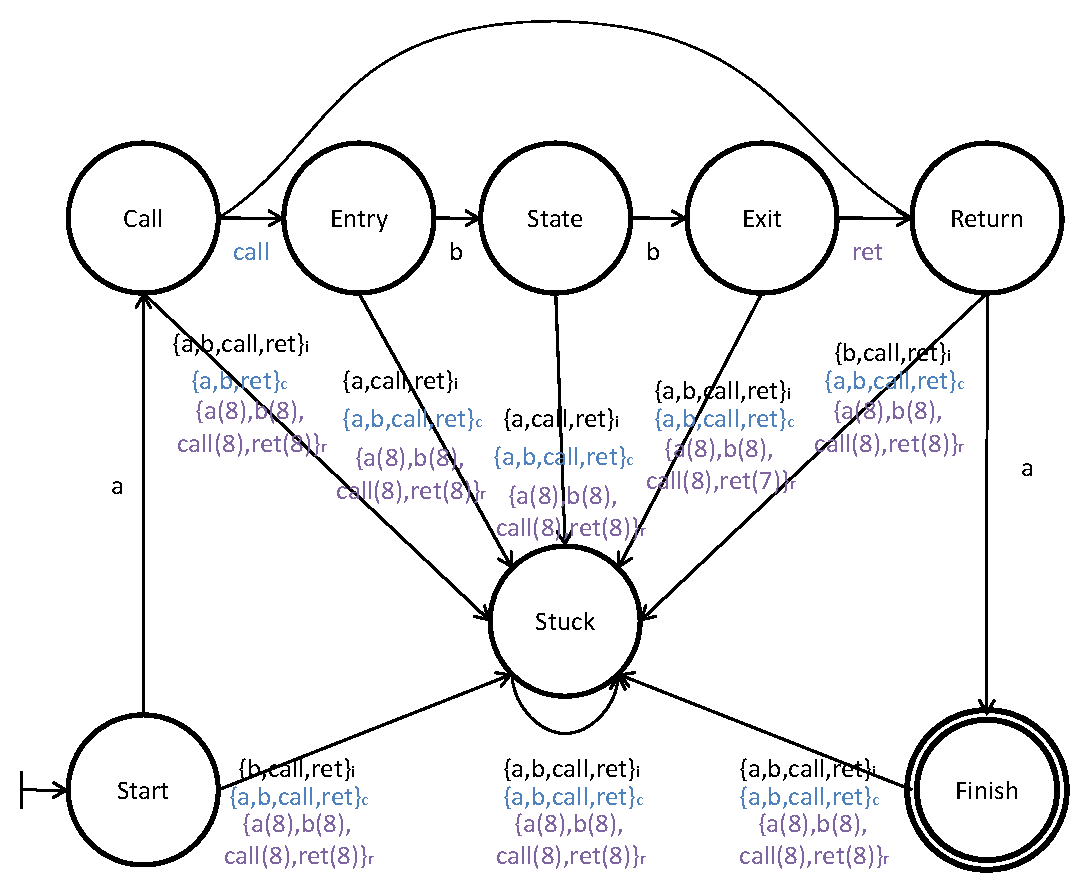
\includegraphics[width=12cm]{Figures/Figure2.eps}
  \caption{An example of an NWA of type 2.  Note: The edge from $Entry$ to $Stuck$ labeled \{a,call,ret\} is a shorthand for three internal transitions in $\delta_i$: $(Entry,a,Stuck)$, $(Entry,call,Stuck)$, and $(Entry,ret,Stuck)$.}
  \label{Fig:Example2}
\end{figure}


\section{Building NWAs from Scratch}
\label{Se:Scratch}

\subsection{States}
\label{Se:States}

The NWA has the possiblility for a special state called the stuck state (recall that an NWA of type 1 has a stuck state).  The stuck state is a state that can never be a final state and has no outgoing transitions except to itself and, to reduce the size of the transition sets of the NWA has implicit incoming transitions.  Any transition to the stuck state, i.e., any internal transition in which the target is the stuck state, any call transition in which the entry state is the stuck state, or any return transition in which the return state is the stuck state, need not be explicitly specified (this occurs only in an NWA of type 1).  In addition, no transition can leave the stuck state unless it is going to the stuck state as well (see Section \ref{Se:Transitions}). \\

\noindent The following operations are methods of class NWA:

\begin{description}

  \item\texttt{Key getStuckState()}

    Allows the user to access the \texttt{Key} for the stuck state.  This method should not be called on an NWA of type 2 because there is no stuck state to retrieve; otherwise there is an assertion violation. 

  \item\texttt{bool isStuckState( Key st )}

    Tests whether the given \texttt{Key}, \texttt{st}, is the stuck state's \texttt{Key}.  If yes, returns true.  Otherwise, returns false. \\

\end{description}

States can be added to an NWA of type 1 individually (using \texttt{addState}, \texttt{addInitialState}, or \texttt{addFinalState}) or as a part of a transition (see Section \ref{Se:Transitions}). Note that in NWAs of type 1, the addition of an individual state automatically introduces an implicit internal transition to the stuck state for each symbol (except meta-symbols, which will be described in greater detail in Section \ref{Se:Symbols}) in the NWA; an implicit call transition to the stuck state for each symbol (except meta-symbols) in the NWA; and two return transitions to the stuck state for each state/symbol pair (except meta-symbols) pair in the NWA, one in which the state added plays the role of the exit state and one in which the state added plays the role of the call state.  Because NWAs of type 2 have no stuck state, such transitions cannot be added automatically and thus adding a state would violate the completeness of the states of the NWA.  Therefore, \textbf{no states can be added to an NWA of type 2}. \\

\noindent The following operations are methods of class NWA:

\begin{description}

  \item\texttt{bool addState( Key st )}

    Adds the given state, \texttt{st}, to $Q$, reporting the success or failure of the addition back to the user in the form of a failure code (returns true for success, returns false for failure).  This method should not be called on an NWA of type 2, otherwise there is an assertion violation.

  \item\texttt{bool addInitialState( Key st )}

    Adds the given state, \texttt{st}, to $Q_0 $ (and also to $Q$ if \texttt{st} $\not\in Q$), reporting the success or failure of the addition back to the user in the form of a failure code (returns true for success, returns false for failure).  This method should not be called on an NWA of type 2, otherwise there is an assertion violation.

  \item\texttt{bool addFinalState( Key st )}

    Adds the given state, \texttt{st}, to $Q_f$ (and also to $Q$ if \texttt{st} $\not\in Q$), reporting the success or failure of the addition back to the user in the form of a failure code (returns true for success, returns false for failure).  If the stuck state is added as a final state, then the NWA is automatically transformed to one of type 2 (by materializing all the implicit transitions) prior to making \texttt{st} a final state.  This method should not be called on an NWA of type 2, otherwise there is an assertion violation. \\

\end{description}


States can be removed from an NWA individually (using \texttt{removeState}) or by clearing the state set of the NWA.  Note that in NWAs of type 1, the removal of an individual state automatically eliminates implicit transitions for each internal transition that has the state being removed as the target, each call transition that has the state being removed as the entry state, and each return transition that has the state being removed as the return state.  Because NWAs of type 2 have no stuck state, such transitions cannot be added automatically and thus removing a state would violate the completeness of the states of the NWA.  Therefore, \textbf{no states can be removed from an NWA of type 2}.  Initial (final) states can be removed from $Q_0 $ ($Q_f$) (but not from $Q$) individually (using \texttt{removeInitialState}, \texttt{removeFinalState}) or by clearing the initial (final) state set of the NWA. \\

\noindent The following operations are methods of class NWA:

\begin{description}

  \item\texttt{bool removeState( Key st )}

    Removes the given state, \texttt{st}, from $Q$ (and also removes \texttt{st} from $Q_0$ if \texttt{st} $\in Q_0$ and removes \texttt{st} from $Q_f$ if \texttt{st} $\in Q_f$), reporting the success or failure of the removal back to the user in the form of a failure code (returns true for success, returns false for failure). This method cannot remove the stuck state from the NWA, because that would create implicit transitions to nowhere.  Any transitions (internal, call, and return) associated with \texttt{st} are also removed from the NWA.  This method should not be called on an NWA of type 2, otherwise there is an assertion violation.

  \item\texttt{void clearStates()}

    Removes all states from $Q$ (including the stuck state).  As a side effect, it also removes all states from $Q_0$ and $Q_f$, as well as all transitions in the NWA.  The symbols in the NWA are not affected.

  \item\texttt{bool removeInitialState( Key st )}

    Removes the given state, \texttt{st}, from $Q_0$ (but not from $Q$ or $Q_f$), reporting the success or failure of the removal back to the user in the form of a failure code (returns true for success, returns false for failure).  Nothing else in the NWA is altered.  This method should not be called on an NWA of type 2, otherwise there is an assertion violation.

  \item\texttt{void clearInitialStates()}

    Removes all states from $Q_0$ (but not from $Q$ or $Q_f$).  Nothing else in the NWA is altered.

  \item\texttt{bool removeFinalState( Key st )}

    Removes the given state, \texttt{st}, from $Q_f$ (but not from $Q$ or $Q_0$), reporting the success or failure of the removal back to the user in the form of a failure code (returns true for success, returns false for failure).  Nothing else in the NWA is altered.  This method should not be called on an NWA of type 2, otherwise there is an assertion violation.

  \item\texttt{void clearFinalStates()}

    Removes all states from $Q_f$ (but not from $Q$ or $Q_0$).  Nothing else in the NWA is altered. \\

\end{description}

The status of individual states (i.e., existence in an NWA, in the initial state set, or in the final state set) can be checked for an NWA of either type (using \texttt{isState}/\texttt{is\_nwa\_state}, \texttt{isInitialState}, and \texttt{isFinalState}).  In addition, states, initial states, and final states can be requested and examined as collections (using \texttt{getStates}/\texttt{get\_states}, \texttt{getInitialStates}, \texttt{getFinalStates}, \texttt{sizeStates}/\texttt{num\_nwa\_states}, \texttt{sizeInitialStates}, and \texttt{sizeFinalStates}). \\

\noindent The following operations are methods of class NWA:

\begin{description}

  \item\texttt{bool isState( Key st ) const}

    Tests whether the given \texttt{Key}, \texttt{st}, is a state in the NWA.  If yes, returns true.  Otherwise, returns false.

  \item\texttt{bool is\_nwa\_state( Key st ) const}

    Same as \texttt{isState}.

  \item\texttt{bool isInitialState( Key st ) const}

    Tests whether the given \texttt{Key}, \texttt{st}, is an initial state in the NWA.  If yes, returns true.  Otherwise, returns false.

  \item\texttt{bool isFinalState( Key st ) const}

    Tests whether the given \texttt{Key}, \texttt{st}, is a final state in the NWA.  If yes, returns true.  Otherwise, returns false.

  \item\texttt{const set<Key>\& getStates() const}

    Returns a \texttt{set} consisting of the \texttt{Keys} of all states in the NWA.

  \item\texttt{const set<Key>\& get\_states() const}

    Same as \texttt{getStates}.

  \item\texttt{const set<Key>\& getInitialStates() const}

    Returns a \texttt{set} consisting of the \texttt{Keys} of all initial states in the NWA.

  \item\texttt{const set<Key>\& getFinalStates() const}

    Returns a \texttt{set} consisting of the \texttt{Keys} of all final states in the NWA.

  \item\texttt{size\_t sizeStates() const}

    Yields the number of states in the NWA.  If the NWA is of type 1, this count includes the stuck state.

  \item\texttt{size\_t num\_nwa\_states() const}

    Same as \texttt{sizeStates}.

  \item\texttt{size\_t sizeInitialStates() const}

    Yields the number of initial states in the NWA.

  \item\texttt{size\_t sizeFinalStates() const}

    Yields the number of final states in the NWA. \\

\end{description}

Each state in the NWA can be associated with some client-specific information. To utilize this functionality, the user must create a subclass of the \texttt{ClientInfo} class (making sure to supply a copy constructor for the subclass).  In addition, the helper methods for intersection and determinization in the \texttt{NWA} class (\texttt{intersectClientInfoInternal}, \texttt{mergeClientInfoInternal}, etc.) must be over-ridden (see Section \ref{Se:Intersection} and Section \ref{Se:Determinize}).  Client information can then be associated with each state in the NWA (using \texttt{setClientInfo}) and accessed given the associated state (using \texttt{getClientInfo}).  For details on automatic generation of client information in NWA operations, see Section \ref{Se:Building NWAs}. \\  

\noindent The following operations are methods of class NWA:

\begin{description}

  \item\texttt{ref\_ptr<ClientInfo> getClientInfo( Key st ) const}

    Allows the user to access the client-specific information associated with the given state, \texttt{st}.

  \item\texttt{void setClientInfo( Key st, const ref\_ptr<ClientInfo> ci )}

    Allows the user to specify the client-specific information, \texttt{ci}, associated with the given state, \texttt{st}. \\

\end{description}

\subsection{Symbols}
\label{Se:Symbols}

The system supports two meta-symbols: \begin{inparaenum} \item \texttt{Epsilon} (\texttt{$\epsilon$}) and \item \texttt{Wild} (\texttt{*}) \end{inparaenum} which are globally available.  \texttt{Epsilon} is the `absence' of a symbol, it denotes the situation in which a transition can be traversed without matching and consuming an input symbol.  \texttt{Epsilon} symbols cannot label call or return transitions (see Section \ref{Se:Transitions}).  \texttt{Wild} is the `any' symbol, it denotes the situation in which a transition can be traversed by consuming a single input symbol of any kind.  Note: \textbf{\texttt{Epsilon} and \texttt{Wild} are not elements of $\Sigma$.} Let $\Sigma^* = \Sigma \cup \{*, \epsilon\}$.\\  

\noindent The following operations are methods of class NWA:

\begin{description}

  \item\texttt{Key getEpsilon()}

    Allows the user to access the \texttt{Key} for the \texttt{Epsilon} meta-symbol.

  \item\texttt{bool isEpsilon( Key sym )}

    Tests whether the given \texttt{Key}, \texttt{sym}, is the \texttt{Key} for the \texttt{Epsilon} meta-symbol.  If yes, returns true.  Otherwise, returns false.

  \item\texttt{Key getWild()}

    Allows the user to access the \texttt{Key} for the \texttt{Wild} meta-symbol.

  \item\texttt{bool isWild( Key sym )}
 
    Tests whether the given \texttt{Key}, \texttt{sym}, is the \texttt{Key} for the \texttt{Wild} meta-symbol. If yes, returns true.  Otherwise, returns false. \\

\end{description}

Symbols can be added to an NWA of type 1 individually (using \texttt{addSymbol}) or as a part of a transition (see Section \ref{Se:Transitions}).  Note that in NWAs of type 1, the addition of a symbol adds an implicit internal transition from each state to the stuck state on the symbol being added, an implicit call transition from each state to the stuck state on the symbol being added, and an implicit return transition from each pair of states to the stuck state on the symbol being added.  Because NWAs of type 2 have no stuck state, such transitions cannot be added automatically and thus adding a symbol would violate the completeness of the states of the NWA.  Therefore, \textbf{no symbols can be added to an NWA of type 2}. \\
 
\noindent The following operations are methods of class NWA:

\begin{description}

  \item\texttt{bool addSymbol( Key sym )}

    Adds the given symbol, \texttt{sym}, to $\Sigma$, reporting the success or failure of the addition back to the user in the form of a failure code (returns true for success, returns false for failure).  Note: \texttt{Wild} and \texttt{Epsilon} are meta-symbol, not symbols of the alphabet, so if \texttt{sym} is the \texttt{Key} for either of these a failure code of false is returned.  This method should not be called on an NWA of type 2, otherwise there is an assertion violation. \\

\end{description}

Symbols can only be removed from an NWA of either type individually (using \texttt{removeSymbol}) or by clearing the alphabet of the NWA (using \texttt{clearSymbols}).  Note that the removal of a symbol removes all internal, call, and return transitions having that symbol (both implicit and explicit) from each state, thus preserving the completeness of the states of the NWA. \\ 

\noindent The following operations are methods of class NWA:

\begin{description}

  \item\texttt{bool removeSymbol( Key sym )}

    Removes the given symbol, \texttt{sym}, from $\Sigma$, reporting the success or failure of the removal back to the user in the form of a failure code (returns true for success, returns false for failure).  Any transitions associated with this symbol are also removed, but no states are altered.  Note: \texttt{Wild} and \texttt{Epsilon} are meta-symbols, not symbols of the alphabet, so if \texttt{sym} is the \texttt{Key} for either of these a failure code of false is returned. 

  \item\texttt{void clearSymbols()}

    Removes all symbols from $\Sigma$.  As a side effect it also removes all transitions in the NWA.  The state set is unaffected. \\

\end{description}

The status of individual symbols (i.e., existence in an NWA) can be checked for an NWA of either type (using \texttt{isSymbol}).  In addition, symbols can be requested and examined as a collection (using \texttt{getSymbols} and \texttt{sizeSymbols}). \\

\noindent The following operations are methods of class NWA:

\begin{description}

  \item\texttt{bool isSymbol( Key sym ) const}

    Tests whether the given \texttt{Key}, \texttt{sym}, is a symbol in the NWA.  If yes, returns true.  Otherwise, returns false.  Note: \texttt{Wild} and \texttt{Epsilon} are meta-symbols, not symbols of the alphabet, so if \texttt{sym} is the \texttt{Key} for either of these false is returned.

  \item\texttt{const set<Key>\& getSymbols() const}

    Returns a \texttt{set} consisting of the \texttt{Keys} of all symbols in the NWA.  Note this does not include meta-symbols.

  \item\texttt{size\_t sizeSymbols() const}

    Yields the number of symbols in the NWA.  This count does not include the meta-symbols \texttt{$\epsilon$} and \texttt{*} even if they have been used in transitions added to the NWA. \\

\end{description}

\subsection{Transitions}
\label{Se:Transitions}

Transitions connect a pair (or triple) of states and are labeled with symbols or meta-symbols.  There are three types of transitions in an NWA: \begin{inparaenum} \item Internal \item Call \item Return. \end{inparaenum}  An internal transition is a transition of the form $(source, sym, target)$ in which $sym$ corresponds to the symbol at an internal position in a nested word accepted by the NWA.  A call transition is a transition of the form $(callSite, sym, entryPoint)$ in which $sym$ corresponds to the symbol at a call position in a nested word accepted by the NWA.  A return transition is a transition of the form $(exitPoint, callSite, sym, returnSite)$ in which $sym$ corresponds to the symbol at a return position in a nested word accepted by the NWA.  The number of transitions of each kind associated with a deterministic NWA is bounded by the number of states and symbols in the NWA.  There can only be $(number\_of\_states)*(number\_of\_symbols)$ internal transitions, $(number\_of\_states)*(number\_of\_symbols)$ call transitions, and $(number\_of\_states)^2*(number\_of\_symbols)$ return transitions.  The number of transitions of each kind associated with a nondeterministic NWA is bounded in a slightly different way by the number of states and symbols in the NWA.  There can only be $(number\_of\_states)^2*(number\_of\_symbols)$ internal transitions, $(number\_of\_states)^2*(number\_of\_symbols)$ call transitions, and $(number\_of\_states)^3*(number\_of\_symbols)$ return transitions.

Transitions can be added to an NWA of type 1 via the overloaded functions \texttt{addInternalTrans}, \texttt{addCallTrans}, and \texttt{addReturnTrans}.  Those functions can either take three \texttt{Keys} that define the transition as input, or an input of type \texttt{KeyTriple\&}.  Alternatively, the set of transitions of a state (or the set of outgoing transitions of a state) can be duplicated for another state (using \texttt{duplicateState} or \texttt{duplicateStateOutgoing}) or all implicit transitions (to the stuck state) can be added as explicit transitions (using \texttt{realizeImplicitTrans}).  As a side effect, if any component (state or symbol) of a transition does not already exist in the NWA it will be added to the NWA.  Thus states and symbols need not be added independently prior to adding transitions.  Note that, in NWAs of type 1, the addition of a state or symbol adds to the NWA implicit transitions to the stuck state (see Section \ref{Se:States} and Section \ref{Se:Symbols}).  Because NWAs of type 2 have no stuck state, such transitions cannot be added automatically, and thus adding a transition would violate the completeness of the states in the NWA.  Therefore, \textbf{no transitions can be added to an NWA of type 2}.  Recall that the stuck state has no outgoing transitions except to itself (see Section \ref{Se:States}).  Thus, no transition leaving the stuck state will be added to the NWA unless it is going to the stuck state as well.  Recall also that the \texttt{$\epsilon$} symbol cannot label a call transition or a return transition (see Section \ref{Se:Symbols}).  Thus, no call or return transition with a symbol of \texttt{$\epsilon$} will be added. \\

\noindent The following operations are methods of class NWA:

\begin{description}

  \item\texttt{bool addInternalTrans( Key source, Key sym, Key target )}

    Adds the internal transition $(\texttt{source},\texttt{sym},\texttt{target})$ to the NWA, reporting the success or failure of the addition back to the user in the form of a failure code (returns true for success, returns false for failure).  In addition, \texttt{source} and \texttt{target} are added as states (if $\texttt{source} \not\in Q$ and $\texttt{target} \not\in Q$, respectively) and \texttt{sym} is added as a symbol (if $\texttt{sym} \not\in \Sigma^*$).  This method should not be called on an NWA of type 2, otherwise there is an assertion violation.

  \item\texttt{bool addInternalTrans( KeyTriple\& intTrans )}

    Adds an internal transition to the NWA for the triple specified by \texttt{intTrans}, reporting the success or failure of the addition back to the user in the form of a failure code (returns true for success, returns false for failure).  In addition, the states of \texttt{intTrans} are added as states of the NWA (if not already states in the NWA) and the symbol of \texttt{intTrans} is added as a symbol of the NWA (if not a meta-symbol or already a symbol in the NWA).  This method should not be called on an NWA of type 2, otherwise there is an assertion violation.

  \item\texttt{bool addCallTrans( Key callSite, Key sym, Key entryPoint )}

    Adds the call transition $(\texttt{callSite},\texttt{sym},\texttt{entryPoint})$ to the NWA, reporting the success or failure of the addition back to the user in the form of a failure code (returns true for success, returns false for failure).  In addition, \texttt{callSite} and \texttt{entryPoint} are added as states of the NWA (if $\texttt{callSite} \not\in Q$ and $\texttt{entryPoint} \not\in Q$, respectively) and \texttt{sym} is added as a symbol of the NWA (if $\texttt{sym} \not\in \Sigma^*$).  This method should not be called on an NWA of type 2, otherwise there is an assertion violation.

  \item\texttt{bool addCallTrans( KeyTriple\& callTrans )}

    Adds a call transition to the NWA for the triple specified by \texttt{callTrans}, reporting the success or failure of the addition back to the user in the form of a failure code (returns true for success, returns false for failure).  In addition, the states of \texttt{callTrans} are added as states of the NWA (if not already states in the NWA) and the symbol of \texttt{callTrans} is added as a symbol of the NWA (if not a meta-symbol or already a symbol in the NWA).  This method should not be called on an NWA of type 2, otherwise there is an assertion violation.

  \item\texttt{bool addReturnTrans( Key exitPoint, Key callSite,\\ \hspace*{3.25cm} Key sym, Key returnSite )}

    Adds the return transition $(\texttt{exitPoint},\texttt{callSite},\texttt{sym},\texttt{returnSite})$ to the NWA, reporting the success or failure of the addition back to the user in the form of a failure code (returns true for success, returns false for failure).  In addition, \texttt{exitPoint}, \texttt{callSite}, and \texttt{returnSite} are added as states of the NWA(if $\texttt{exitPoint} \not\in Q$, $\texttt{callSite} \not\in Q$, and $\texttt{returnSite} \not\in Q$, respectively) and \texttt{sym} is added as a symbol (if $\texttt{sym} \not\in \Sigma^*$).  This method should not be called on an NWA of type 2, otherwise there is an assertion violation.

  \item\texttt{bool addReturnTrans( KeyQuad\& retTrans )}

    Adds a return transition to the NWA for the 4-tuple specified by \texttt{retTrans}, reporting the success or failure of the addition back to the user in the form of a failure code (returns true for success, returns false for failure).  In addition, the states of \texttt{retTrans} are added as states (if not already states in the NWA) and the symbol of \texttt{retTrans} is added as a symbol (if not a meta-symbol or already a symbol in the NWA).  This method should not be called on an NWA of type 2, otherwise there is an assertion violation.

  \item\texttt{void duplicateState( Key orig, Key dup )}

    Duplicates all the transitions containing the state \texttt{orig} and adds the transitions to the NWA with \texttt{orig} replaced by \texttt{dup}.  Self-loops are duplicated by adding a transition to the NWA for all possible combinations of some occurrence of \texttt{orig} replaced by \texttt{dup}, i.e., if $(\texttt{orig},a,\texttt{orig})$ is an internal (or call) transition, then the transitions $(\texttt{dup},a,\texttt{dup})$, $(\texttt{dup},a,\texttt{orig})$, and $(\texttt{orig},a,\texttt{dup})$ are added and if $(\texttt{orig},\texttt{orig},a,\texttt{orig})$ is a return transition, then the transitions $(\texttt{dup},\texttt{dup},a,\texttt{dup})$, $(\texttt{dup},\texttt{dup},a,\texttt{orig})$,  $(\texttt{orig},\texttt{dup},a,\texttt{dup})$, and $(\texttt{orig},\texttt{dup},a,\texttt{orig})$ as well as $(\texttt{dup},\texttt{orig},a,\texttt{dup})$, $(\texttt{dup},\texttt{orig},a,\texttt{orig})$, and $(\texttt{orig},\texttt{orig},a,\texttt{dup})$ are added.  This method should not be called on an NWA of type 2, otherwise there is an assertion violation.

  \item\texttt{void duplicateStateOutgoing( Key orig, Key dup )}

    Duplicates all the transitions originating from \texttt{orig} and adds the transitions to the NWA with \texttt{orig} replaced by \texttt{dup}.  Self-loops are duplicated by adding a transition to the NWA for all possible combinations of some occurrence of \texttt{orig} replaced by \texttt{dup} while maintaining that the transitions are outgoing from \texttt{dup}, i.e., if $(\texttt{orig},a,\texttt{orig})$ is an internal (or call) transition, then the transitions $(\texttt{dup},a,\texttt{dup})$ and $(\texttt{dup},a,\texttt{orig})$ are added and if $(\texttt{orig},\texttt{orig},a,\texttt{orig})$ is a return transition, then the transitions $(\texttt{dup},\texttt{dup},a,\texttt{dup})$ and $(\texttt{dup},\texttt{dup},a,\texttt{orig})$, as well as $(\texttt{dup},\texttt{orig},a,\texttt{dup})$ and $(\texttt{dup},\texttt{orig},a,\texttt{orig})$ are added.  This method should not be called on an NWA of type 2, otherwise there is an assertion violation.

  \item\texttt{void realizeImplicitTrans()}

    Adds all implicit transitions explicitly to the stuck state.  This should only be called on an NWA of type 1 and changes the NWA to an NWA of type 2.  Otherwise there is an assertion violation. \\

\end{description}

Transitions can only be removed from an NWA of type 1 as units or by specifying component parts (using \texttt{removeInternalTrans}, \texttt{removeCallTrans}, or \texttt{removeReturnTrans}), by clearing all transitions from the NWA, or as a side effect of removing a state or symbol from the NWA (see Section \ref{Se:States} and Section \ref{Se:Symbols}).  Note that, in NWAs of type 1, the removal of a transition will add an implicit transition with the same source/call-state/exit- and call- states,the same symbol, and the stuck state as the target/entry-state/return-state.  Because NWAs of type 2 have no stuck state, such transitions cannot be added automatically, and thus removing a transition would violate the completeness of the states in the NWA.  Therefore, \textbf{no transitions can be removed from an NWA of type 2}. \\ 

\noindent The following operations are methods of class NWA:

\begin{description}

  \item\texttt{bool removeInternalTrans( Key source, Key sym, Key target )}

    Removes the internal transition $(\texttt{source},\texttt{sym},\texttt{target})$ from the NWA (if $(\texttt{source},\texttt{sym},\texttt{target}) \in \delta_i$), reporting the success or failure of the removal back to the user in the form of a failure code (returns true for success, returns false for failure).  This method should not be called on an NWA of type 2, otherwise there is an assertion violation.

  \item\texttt{bool removeInternalTrans( KeyTriple\& intTrans )}

    Removes an internal transition from the NWA for the triple specified by \texttt{intTrans} (if \texttt{intTrans} $\in \delta_i$), reporting the success or failure of the removal back to the user in the form of a failure code (returns true for success, returns false for failure).  This method should not be called on an NWA of type 2, otherwise there is an assertion violation.

  \item\texttt{bool removeCallTrans( Key callSite, Key sym, Key entryPoint )}

    Removes the call transition $(\texttt{callSite},\texttt{sym},\texttt{entryPoint})$ from the NWA (if $(\texttt{callSite},\texttt{sym},\texttt{entryPoint}) \in \delta_c$), reporting the success or failure of the removal back to the user in the form of a failure code (returns true for success, returns false for failure).  This method should not be called on an NWA of type 2, otherwise there is an assertion violation. 
 
  \item\texttt{bool removeCallTrans( KeyTriple\& callTrans )}

    Removes a call transition from the NWA for the triple specified by \texttt{callTrans} (if \texttt{callTrans} $\in \delta_c$), reporting the success or failure of the removal back to the user in the form of a failure code (returns true for success, returns false for failure).  This method should not be called on an NWA of type 2, otherwise there is an assertion violation.

  \item\texttt{bool removeReturnTrans( Key exitPoint, Key callSite,\\ \hspace*{3.25cm} Key sym, Key returnSite )}

    Removes the return transition $(\texttt{exitPoint},\texttt{callSite},\texttt{sym},\texttt{returnSite})$ from the NWA (if $(\texttt{exitPoint},\texttt{callSite},\texttt{sym},\texttt{returnSite}) \in \delta_r$), reporting the success or failure of the removal back to the user in the form of a failure code (returns true for success, returns false for failure).  This method should not be called on an NWA of type 2, otherwise there is an assertion violation.

  \item\texttt{bool removeReturnTrans( Key exitPoint, Key sym, Key returnSite )}

    Removes the return transitions $(\texttt{exitPoint},st,\texttt{sym},\texttt{returnSite})$ for all \\$st \in Q$ from the NWA (if $(\texttt{exitPoint},st,\texttt{sym},\texttt{returnSite}) \in \delta_r$), reporting the success or failure of the removal back to the user in the form of a failure code (returns true for success, returns false for failure).  This method should not be called on an NWA of type 2, otherwise there is an assertion violation.

  \item\texttt{bool removeReturnTrans( KeyQuad\& retTrans )}

    Removes a return transition from the NWA for the quadruple specified by \texttt{retTrans} (if \texttt{retTrans} $\in \delta_r$), reporting the success or failure of the removal back to the user in the form of a failure code (returns true for success, returns false for failure).  This method should not be called on an NWA of type 2, otherwise there is an assertion violation.

  \item\texttt{void clearTrans()}

    Removes all transitions from the NWA, but does not remove any states or symbols. \\

\end{description}

The set of supported queries about an NWA's explicit transitions includes: the existence of a specified transition, the number of (internal, call, return, or total) transitions in the NWA, the set of states that are predecessors (sources of internal transitions, call states of call transitions, or exit states of return transitions) of a given state by some transition (with and without a specified symbol), the set of states that are call predecessors of a given state by some return transition (with and without a specified symbol), the set of states that are successors (targets of internal transitions, entry states of call transitions, or return states of return transitions) of a given state by some transition (with and without a specified symbol), the set of states that are successors of a given call predecessor (return states) by some return transition (with and without a specified symbol), the set of symbol/state pairs for which there exist internal transitions with a particular source, the set of symbol/state pairs for which there exist call transitions with a particular call state, the set of symbol/state pairs for which there exist return transitions with a particular exit state and call state, the set of sources that are associated with a given target, the set of targets that are associated with a given source, the set of call states that are associated with a given entry state, the set of entry states that are associated with a given call state, the set of exit states that are assoicated with a given call state, the set of exit states that are assoicated with a given return state, the set of call states that are associated with a given exit state, the set of call states that are associated with a given return state, the set of return states that are associated with a given exit state, the set of return states that are associated with a given call state, etc. \\

\noindent The following operations are methods of class NWA:

\begin{description}

  \item\texttt{bool findTrans( Key from, Key sym, Key to )}

    Tests whether there exists an internal transition $(\texttt{from},\texttt{sym},\texttt{to}) \in \delta_i$, a call transition $(\texttt{from},\texttt{sym},\texttt{to}) \in \delta_c$, or a return transition $(\texttt{from},st,\texttt{sym},\texttt{to}) \in \delta_r$ for some $st \in Q$.

  \item\texttt{bool getSymbol( Key from, Key to, Key\& sym )}

    Tests whether there exists an internal transition $(\texttt{from},\alpha,\texttt{to}) \in \delta_i$ for some $\alpha \in \Sigma^*$, a call transition $(\texttt{from},\alpha,\texttt{to}) \in \delta_c$ for some $\alpha \in \Sigma \cup \{*\}$, or a return transition $(\texttt{from},st,\alpha,\texttt{to}) \in \delta_r$ for some $st \in Q$ and some $\alpha \in \Sigma \cup \{*\}$.  In addition, the $\alpha$ for the first such transition found is stored in the reference parameter \texttt{sym}.

  \item\texttt{size\_t sizeInternalTrans()}

    Yields the number of explicit internal transitions in the NWA.

  \item\texttt{size\_t sizeCallTrans()}

    Yields the number of explicit call transitions in the NWA.

  \item\texttt{size\_t sizeReturnTrans()}

    Yields the number of explicit return transitions in the NWA.

  \item\texttt{size\_t sizeTrans()}

    Yields the total number of explicit transitions (internal, call, and return) in the NWA.

  \item\texttt{int count\_rules()}

    Same as \texttt{sizeTrans}.

  \item\texttt{const std::set<Key> getPredecessors( Key state )}

    Yields all states that are predecessors of a given state by some transition; i.e., for each internal transition, $(source,sym,\texttt{state})$, $source$ is added to the set of predecessors, for each call transition, $(callSite,sym,\texttt{state})$, $callSite$ is added to the set of predecessors, and for each return transition, $(exitPoint,callSite,sym,\texttt{state})$, $exitPoint$ is added to the set of predecessors.

  \item\texttt{const std::set<Key> getPredecessors( Key symbol, Key state )}

    Yields all states that are predecessors of a given state by some transition having the given symbol; i.e., for each internal transition, $(source,\texttt{symbol},\texttt{state})$, $source$ is added to the set of predecessors, for each call transition, $(callSite,\texttt{symbol},\texttt{state})$, $callSite$ is added to the set of predecessors, and for each return transition, $(exitPoint,callSite,\texttt{symbol},\texttt{state})$, $exitPoint$ is added to the set of predecessors.

  \item\texttt{const std::set<Key> getSuccessors( Key state )}

    Yields all states that are successors of a given state by some transition; i.e., for each internal transition, $(\texttt{state},sym,target)$, $target$ is added to the set of successors, for each call transition, $(\texttt{state},sym,entryPoint)$, $entryPoint$ is added to the set of successors, and for each return transition, $(\texttt{state},callSite,sym,returnSite)$, $returnSite$ is added to the set of successors.

  \item\texttt{const std::set<Key> getSuccessors( Key state, Key symbol )}

    Yields all states that are successors of a given state by some transition having the given symbol; i.e., for each internal transition, $(\texttt{state},\texttt{symbol},target)$, $target$ is added to the set of successors, for each call transition, $(\texttt{state},\texttt{symbol},entryPoint)$, $entryPoint$ is added to the set of successors, and for each return transition, $(\texttt{state},callSite,\texttt{symbol},returnSite)$, $returnSite$ is added to the set of successors.

  \item\texttt{const std::set<Key> getCallPredecessors( Key state )}

    Yields all states that are call-predecessors of a given state by some return transition; i.e., for each return transition, $(exitPoint,callSite,sym,\texttt{state})$, $callSite$ is added to the set of call predecessors.

  \item\texttt{const std::set<Key> getCallPredecessors( Key symbol, Key state )}

    Yields all states that are call-predecessors of a given state by some return transition having the given symbol; i.e., for each return transition, $(exitPoint,callSite,\texttt{symbol},\texttt{state})$, $callSite$ is added to the set of call predecessors.

  \item\texttt{const std::set<Key> getCallSuccessors( Key state )}

    Yields all states that are call-successors of a given state by some return transition; i.e., for each return transition, $(exitPoint,\texttt{state},sym,returnSite)$, $returnSite$ is added to the set of call successors.

  \item\texttt{const std::set<Key> getCallSuccessors( Key state, Key symbol )}

    Yields all states that are call-successors of a given state by some return transition having the given symbol; i.e., for each return transition, $(exitPoint,\texttt{state},\texttt{symbol},returnSite)$, $returnSite$ is added to the set of call successors.

  \item\texttt{const std::set<Key> getSources\_Sym( Key symbol )}

    Yields the set of all states, $source$, such that the internal transition $(source,\texttt{symbol},target) \in \delta_i$ for some $target \in Q$.

  \item\texttt{const std::set<Key> getSources( Key symbol, Key target )}

    Yields the set of all states, $source$, such that the internal transition $(source,\texttt{symbol},\texttt{target}) \in \delta_i$.

  \item\texttt{const std::set<std::pair<Key,Key>> getSources( Key target )}

    Yields the set of all state/symbol pairs, $(source,sym)$, such that the internal transition $(source,sym,\texttt{target}) \in \delta_i$.

  \item\texttt{const std::set<Key> getSources( )}

    Yields the set of all states, $source$, such that the internal transition $(source,symbol,target) \in \delta_i$ for some $symbol \in \Sigma$ and $target \in Q$.

  \item\texttt{const std::set<Key> getTargets\_Sym( Key symbol )}

    Yields the set of all states, $target$, such that the internal transition $(source,\texttt{symbol},target) \in \delta_i$ for some $source \in Q$.

  \item\texttt{const std::set<Key> getTargets( Key source, Key symbol )}

    Yields the set of all states, $target$, such that the internal transition $(\texttt{source},\texttt{symbol},target) \in \delta_i$.

  \item\texttt{const std::set<std::pair<Key,Key>> getTargets( Key source )}

    Yields the set of all symbol/state pairs, $(sym,target)$, such that the internal transition $(\texttt{source},sym,target) \in \delta_i$.

  \item\texttt{const std::set<Key> getTargets( )}

    Yields the set of all states, $target$, such that the internal transition $(source,symbol,target) \in \delta_i$ for some $source \in Q$ and $symbol \in \Sigma$.

  \item\texttt{const std::set<Key> getInternalSym( )}

    Yields the set of all symbols, $symbol$, such that the internal transition $(source,symbol,target) \in \delta_i$ for some $source \in Q$ and $target \in Q$.

  \item\texttt{const std::set<Key> getInternalSym( Key source, Key target )}

    Yields the set of all symbols, $symbol$, such that the internal transition $(\texttt{source},symbol,\texttt{target}) \in \delta_i$.

  \item\texttt{const std::set<Key> getInternalSym\_Source( Key source )}

    Yields the set of all symbols, $symbol$, such that the internal transition $(\texttt{source},symbol,target) \in \delta_i$ for some $target \in Q$.

  \item\texttt{const std::set<Key> getInternalSym\_Target( Key target )}

    Yields the set of all symbols, $symbol$, such that the internal transition $(source,symbol,\texttt{target}) \in \delta_i$ for some $source \in Q$.

  \item\texttt{const std::set<Key> getCallSites\_Sym( Key symbol )}

    Yields the set of all states, $callSite$, such that the call transition $(callSite,\texttt{symbol},entryPoint) \in \delta_c$ for some $entryPoint \in Q$.

  \item\texttt{const std::set<Key> getCallSites( Key symbol, Key entryPoint )}

    Yields the set of all states, $callSite$, such that the call transition $(callSite,\texttt{symbol},\texttt{entryPoint}) \in \delta_c$.

  \item\texttt{const std::set<std::pair<Key,Key>> getCallSites( Key entryPoint )}

    Yields the set of all state/symbol pairs, $(callSite,sym)$, such that $(callSite,sym,entryPoint) \in \delta_c$. 

  \item\texttt{const std::set<Key> getCallSites( )}

    Yields the set of all states, $callSite$, such that $(callSite,symbol,entryPoint) \in \delta_c$ for some $symbol \in \Sigma$ and $entryPoint \in Q$.

  \item\texttt{const std::set<Key> getEntries\_Sym( Key symbol )}

    Yields the set of all states, $entryPoint$, such that $(callSite,\texttt{symbol},entryPoint) \in \delta_c$ for some $callSite \in Q$.

  \item\texttt{const std::set<Key> getEntries( Key callSite, Key symbol )}

    Yields the set of all states, $entryPoint$, such that the call transition $(\texttt{callSite},\texttt{symbol},entryPoint) \in \delta_c$.

  \item\texttt{const std::set<std::pair<Key,Key>> getEntries( Key callSite )}

    Yields the set of all symbol/state pairs, $(sym,entryPoint)$, such that the call transition $(\texttt{callSite},sym,entryPoint) \in \delta_c$.

  \item\texttt{const std::set<Key> getEntries( )}

    Yields the set of all states, $entryPoint$, such that the call transition $(callSite,symbol,entryPoint) \in \delta_c$ for some $callSite \in Q$ and $symbol \in \Sigma$.

  \item\texttt{const std::set<Key> getCallSym( )}

    Yields the set of all symbols, $symbol$, such that the call transition $(callSite,symbol,entryPoint) \in \delta_c$ for some $callSite \in Q$ and $entryPoint \in Q$.

  \item\texttt{const std::set<Key> getCallSym( Key callSite, Key entryPoint )}

    Yields the set of all symbols, $symbol$, such that the call transition $(\texttt{callSite},symbol,\texttt{entryPoint}) \in \delta_c$.

  \item\texttt{const std::set<Key> getCallSym\_Call( Key callSite )}

    Yields the set of all symbols, $symbol$, such that the call transition $(\texttt{callSite},symbol,entryPoint) \in \delta_c$ for some $entryPoint \in Q$.

  \item\texttt{const std::set<Key> getCallSym\_Entry( Key entryPoint )}

    Yields the set of all symbols, $symbol$, such that the call transition $(callSite,symbol,\texttt{entryPoint}) \in \delta_c$ for some $callSite \in Q$.

  \item\texttt{const std::set<Key> getExits\_Sym( Key symbol )}

    Yields the set of all states, $exitPoint$, such that the return transition $(exitPoint,callSite,\texttt{symbol},returnSite) \in \delta_r$ for some $callSite \in Q$ and $returnSite \in Q$.

  \item\texttt{const std::set<Key> getExits( Key callSite, Key symbol,\\ \hspace*{3.25cm} Key returnSite )}

    Yields the set of all states, $exitPoint$, such that the return transition $(exitPoint,\texttt{callSite},\texttt{symbol},\texttt{returnSite}) \in \delta_r$.

  \item\texttt{const std::set<std::pair<Key,Key>> getExits( Key callSite,\\ \hspace*{3.25cm} Key returnSite )}

    Yields the set of all state/symbol pairs, $(exitPoint,sym)$, such that the return transition $(exitPoint,\texttt{callSite},sym,\texttt{returnSite}) \in \delta_r$.

  \item\texttt{const std::set<Key> getExits( )}

    Yields the set of all states, $exitPoint$, such that the return transition $(exitPoint,callSite,symbol,returnSite) \in \delta_r$ for some $callSite \in Q$, $symbol \in \Sigma$, and $returnSite \in Q$.

  \item\texttt{const std::set<Key> getExits\_Call( Key callSite, Key symbol )}

    Yields the set of all states, $exitPoint$, such that the return transition $(exitPoint,\texttt{callSite},\texttt{symbol},returnSite) \in \delta_r$ for some $returnSite \in Q$.

  \item\texttt{const std::set<std::pair<Key,Key>> getExits\_Call( Key callSite )}

    Yields the set of all state/symbol pairs, $(exitPoint,sym)$, such that the return transition $(exitPoint,\texttt{callSite},sym,returnSite) \in \delta_r$ for some $returnSite \in Q$.

  \item\texttt{const std::set<Key> getExits\_Ret( Key symbol, Key returnSite )}

    Yields the set of all states, $exitPoint$, such that the return transition $(exitPoint,callSite,\texttt{symbol},\texttt{returnSite}) \in \delta_r$ for some $callSite \in Q$.

  \item\texttt{const std::set<std::pair<Key,Key>> getExits\_Ret( Key returnSite )}

    Yields the set of all state/symbol pairs, $(exitPoint,sym)$, such that the return transition $(exitPoint,callSite,sym,\texttt{returnSite}) \in \delta_r$ for some $callSite \in Q$.

  \item\texttt{const std::set<Key> getCalls\_Sym( Key symbol )}

    Yields the set of all states, $callSite$, such that the return transition $(exitPoint,callSite,\texttt{symbol},returnSite) \in \delta_r$ for some $exitPoint \in Q$ and $returnSite \in Q$.

  \item\texttt{const std::set<Key> getCalls( Key exitPoint, Key symbol,\\ \hspace*{3.25cm} Key returnSite )}

    Yields the set of all states, $callSite$, such that the return transition $(\texttt{exitPoint},callSite,\texttt{symbol},\texttt{returnSite}) \in \delta_r$.

  \item\texttt{const std::set<std::pair<Key,Key>> getCalls( Key exitPoint,\\ \hspace*{3.25cm} Key returnSite )}

    Yields the set of all state/symbol pairs, $(callSite,sym)$, such that the return transition $(\texttt{exitPoint},callSite,sym,\texttt{returnSite} \in \delta_r$.

  \item\texttt{const std::set<Key> getCalls( )}

    Yields the set of all states, $callSite$, such that the return transition $(exitPoint,callSite,symbol,returnSite) \in \delta_r$ for some $exitPoint \in Q$, $symbol \in \Sigma$, and $returnSite \in Q$.

  \item\texttt{const std::set<Key> getCalls\_Exit( Key exitPoint, Key symbol )}

    Yields the set of all states, $callSite$, such that the return transition $(\texttt{exitPoint},callSite,\texttt{symbol},returnSite) \in \delta_r$ for some $returnSite \in Q$.

  \item\texttt{const std::set<std::pair<Key,Key>> getCalls\_Exit( Key exitPoint )}

    Yields the set of all state/symbol pairs, $(callSite,sym)$, such that the return transition $(\texttt{exitPoint},callSite,sym,returnSite) \in \delta_r$ for some $returnSite \in Q$.

  \item\texttt{const std::set<Key> getCalls\_Ret( Key symbol, Key returnSite )}

    Yields the set of all states, $callSite$, such that the return transition $(exitPoint,callSite,\texttt{symbol},\texttt{returnSite} \in \delta_r$ for some $exitPoint \in Q$.

  \item\texttt{const std::set<std::pair<Key,Key>> getCalls\_Ret( Key returnSite )}

    Yields the set of all state/symbol pairs, $(callSite,sym)$, such that the return transition $(exitPoint,callSite,sym,\texttt{returnSite} \in \delta_r$ for some $exitPoint \in Q$.

  \item\texttt{const std::set<Key> getReturns\_Sym( Key symbol )}

    Yields the set of all states, $returnSite$, such that the return transition $(exitPoint,callSite,\texttt{symbol},returnSite) \in \delta_r$ for some $exitPoint \in Q$ and $callSite \in Q$.

  \item\texttt{const std::set<Key> getReturns( Key exitPoint ,Key callSite,\\ \hspace*{3.25cm} Key symbol )}

    Yields the set of all states, $returnSite$, such that the return transition $(\texttt{exitPoint},\texttt{callSite},\texttt{symbol},returnSite) \in \delta_r$.

  \item\texttt{const std::set<std::pair<Key,Key>> getReturns( Key exitPoint,\\ \hspace*{3.25cm} Key callSite )}

    Yields the set of all symbol/state pairs, $(sym,returnSite)$, such that the return transition $(\texttt{exitPoint},\texttt{callSite},sym,returnSite) \in \delta_r$.

  \item\texttt{const std::set<Key> getReturns( )}

    Yields the set of all states, $returnSite$, such that the return transition $(exitPoint,callSite,symbol,returnSite) \in \delta_r$ for some $exitPoint \in Q$, $callSite \in Q$, and $symbol \in \Sigma$.

  \item\texttt{const std::set<Key> getReturns\_Exit( Key exitPoint, Key symbol )}

    Yields the set of all states, $returnSite$, such that the return transition $(\texttt{exitPoint},callSite,\texttt{symbol},returnSite) \in \delta_r$ for some $callSite \in Q$.

  \item\texttt{const std::set<std::pair<Key,Key>> \\getReturns\_Exit( Key exitPoint )}

    Yields the set of all symbol/state pairs, $(sym,returnSite)$, such that the return transition $(\texttt{exitPoint},callSite,sym,returnSite) \in \delta_r$ for some $callSite \in Q$.

  \item\texttt{const std::set<Key> getReturns\_Call( Key callSite, Key symbol )}

    Yields the set of all states, $returnSite$, such that the return transition $(exitPoint,\texttt{callSite},\texttt{symbol},returnSite) \in \delta_r$ for some $exitPoint \in Q$.

  \item\texttt{const std::set<std::pair<Key,Key>> getReturns\_Call( \\ \hspace*{3.25cm} Key callSite )}

    Yields the set of all symbol/state pairs, $(sym,returnSite)$, such that the return transition $(exitPoint,\texttt{callsite},sym,returnSite) \in \delta_r$ for some $exitPoint \in Q$.

  \item\texttt{const std::set<Key> getReturnSites( Key callSite )}

    Yields the set of all states, $returnSite$, such that the return transition $(exitPoint,\texttt{callSite},sym,returnSite) \in \delta_r$ for some $exitPoint \in Q$ and $sym \in \Sigma$.

  \item\texttt{const std::set<Key> getReturnSym( \\ \hspace*{3.25cm}Key exitPoint, Key callSite, Key returnSite )}

    Yields the set of all symbols, $symbol$, such that the return transition $(\texttt{exitPoint},\texttt{callSite},symbol,\texttt{returnSite}) \in \delta_r$.

  \item\texttt{const std::set<Key> getReturnSym( )}

    Yields the set of all symbols, $symbol$, such that the return transition $(exitPoint,callSite,symbol,returnSite) \in \delta_r$ for some $exitPoint \in Q$, $callSite \in Q$, and $returnSite \in Q$.

  \item\texttt{const std::set<Key> getReturnSym\_Exit( Key exitPoint )}

    Yields the set of all symbols, $symbol$, such that the return transition $(\texttt{exitPoint},callSite,symbol,returnSite) \in \delta_r$ for some $callSite \in Q$ and $returnSite \in Q$.

  \item\texttt{const std::set<Key> getReturnSym\_Call( Key callSite )}

    Yields the set of all symbols, $symbol$, such that the return transition $(exitPoint,\texttt{callSite},symbol,returnSite) \in \delta_r$ for some $exitPoint \in Q$ and $returnSite \in Q$.

  \item\texttt{const std::set<Key> getReturnSym\_Ret( Key returnSite )}

    Yields the set of all symbols, $symbol$, such that the return transition $(exitPoint,callSite,symbol,\texttt{returnSite}) \in \delta_r$ for some $exitPoint \in Q$ and $callSite \in Q$.

  \item\texttt{const std::set<Key> getReturnSym\_ExitCall( \\ \hspace*{3.25cm} Key exitPoint, Key callSite )}

    Yields the set of all symbols, $symbol$, such that the return transition $(\texttt{exitPoint}\texttt{callSite},symbol,returnSite) \in \delta_r$ for some $returnSite \in Q$.

  \item\texttt{const std::set<Key> getReturnSym\_ExitRet( \\ \hspace*{3.25cm} Key exitPoint, Key returnSite )}

    Yields the set of all symbols, $symbol$, such that the return transition $(\texttt{exitPoint},callSite,symbol,\texttt{returnSite}) \in \delta_r$ for some $callSite \in Q$.

  \item\texttt{const std::set<Key> getReturnSym\_CallRet( \\ \hspace*{3.25cm} Key callSite, Key returnSite )}

    Yields the set of all symbols, $symbol$, such that the return transition $(exitPoint,\texttt{callSite},symbol,\texttt{returnSite}) \in \delta_r$ for some $exitPoint \in Q$. \\

\end{description}

\section{Building NWAs from other NWAs}
\label{Se:Building NWAs}

NWAs do not need to be built state by state and transition by transition, they can also be built by performing language-theoretic operations over component NWAs. These operations include: union, intersection, concatenation, reversal, Kleene-star, complement, and determinize. The library supports two interfaces to the Boolean operations.  In one, each operation returns a \texttt{ref\_ptr<NWA>} to a freshly built NWA.  In the other, each operation transforms the NWA on which it was called. \\

\noindent The following operations are methods of class NWA:

\begin{description}

  \item\texttt{static ref\_ptr<NWA> unionNWA(  \\ \hspace*{3.25cm} ref\_ptr<NWA> first, ref\_ptr<NWA> second, \\ \hspace*{3.25cm} Key stuck )}

    The result is the union of the NWAs \texttt{first} and \texttt{second}.  The stuck state of the resulting NWA is \texttt{stuck}.  See Section \ref{Se:Union}.  

  \item\texttt{static ref\_ptr<NWA> intersect(  \\ \hspace*{3.25cm} ref\_ptr<NWA> first, ref\_ptr<NWA> second, \\ \hspace*{3.25cm} Key stuck )}

    The result is the intersection of the NWAs \texttt{first} and \texttt{second}.  The stuck state of the resulting NWA is \texttt{stuck}.  See Section \ref{Se:Intersection}.

  \item\texttt{static ref\_ptr<NWA> concat(  \\ \hspace*{3.25cm} ref\_ptr<NWA> first, ref\_ptr<NWA> second, \\ \hspace*{3.25cm} Key stuck )}

    The result is the concatenation of the NWAs \texttt{first} and \texttt{second}.  The stuck state of the resulting NWA is \texttt{stuck}.  See Section \ref{Se:Concatenation}.

  \item\texttt{static ref\_ptr<NWA> star( ref\_ptr<NWA> first, Key stuck )}

    The result is the Kleene-Star of the NWA \texttt{first}.  The stuck state of the resulting NWA is \texttt{stuck}.  See Section \ref{Se:Star}.

  \item\texttt{static ref\_ptr<NWA> reverse( ref\_ptr<NWA> first, Key stuck )}

    The result is the NWA which accepts the reverse of each nested word accepted by the NWA \texttt{first}.  The stuck state of the resulting NWA is \texttt{stuck}.  See Section \ref{Se:Reverse}.

  \item\texttt{static ref\_ptr<NWA> determinize( ref\_ptr<NWA> nondet, Key stuck )}

    The result is the deterministic NWA that is equivalent to the NWA \texttt{nondet}.  The stuck state of the resulting NWA is \texttt{stuck}.  See Section \ref{Se:Determinize}.

  \item\texttt{static ref\_ptr<NWA> complement( ref\_ptr<NWA> first, Key stuck )}

    The result is the NWA which is the complement of the NWA \texttt{first}.  The stuck state of the resulting NWA is \texttt{stuck}.  See Section \ref{Se:Complement}.

  \item\texttt{void unionNWA( ref\_ptr<NWA> first, ref\_ptr<NWA> second )}

    This operation is an NWA method; the NWA referred to by \texttt{this} is transformed into the NWA resulting from the union of the NWAs \texttt{first} and \texttt{second}.  See Section \ref{Se:Union}.  This method should not be called on an NWA of type 2, otherwise there is an assertion violation.  Typical sequence of operations: construct A; A.unionNWA(B,C);

 \item\texttt{void intersect( ref\_ptr<NWA> first, ref\_ptr<NWA> second )}

    This operation is an NWA method; the NWA referred to by \texttt{this} is transformed into the NWA resulting from the intersection of the NWAs \texttt{first} and \texttt{second}.  See Section \ref{Se:Intersection}.  This method should not be called on an NWA of type 2, otherwise there is an assertion violation.  Typical sequence of operations: construct A; A.intersect(B,C);

  \item\texttt{void concat( ref\_ptr<NWA> first, ref\_ptr<NWA> second )}

    This operation is an NWA method; the NWA referred to by \texttt{this} is transformed into the NWA resulting from concatenating the NWAs \texttt{first} and \texttt{second}.  See Section \ref{Se:Concatenation}.  This method should not be called on an NWA of type 2, otherwise there is an assertion violation.  Typical sequence of operations: construct A; A.concat(B,C);

  \item\texttt{void star( ref\_ptr<NWA> first )}

    This operation is an NWA method; the NWA referred to by \texttt{this} is transformed into the NWA resulting from performing the Kleene-Star operation on the NWA \texttt{first}.  See Section \ref{Se:Star}.  This method should not be called on an NWA of type 2, otherwise there is an assertion violation.  Typical sequence of operations: construct A; A.star(B);

  \item\texttt{void reverse( ref\_ptr<NWA> first )}

    This operation is an NWA method; the NWA referred to by \texttt{this} is transformed into the NWA which accepts the reverse of each nested word accepted by the NWA \texttt{first}.  See Section \ref{Se:Reverse}.  This method should not be called on an NWA of type 2, otherwise there is an assertion violation.  Typical sequence of operations: construct A; A.reverse(B);

  \item\texttt{void determinize( ref\_ptr<NWA> nondet )}

    This operation is an NWA method; the NWA referred to by \texttt{this} is transformed into the deterministic NWA that is equivalent to the NWA \texttt{nondet}.  See Section \ref{Se:Determinize}.  This method should not be called on an NWA of type 2, otherwise there is an assertion violation.  Typical sequence of operations: construct A; A.determinize(B);

  \item\texttt{void complement( ref\_ptr<NWA> first )}

    This operation is an NWA method; the NWA referred to by \texttt{this} is transformed into the NWA resulting from complementing the NWA \texttt{first}.  See Section \ref{Se:Complement}.  This method should not be called on an NWA of type 2, otherwise there is an assertion violation.  Typical sequence of operations: construct A; A.complement(B);

\end{description}

\subsection{Union}
\label{Se:Union}
Consider an example of computing the union of two NWAs, the NWA shown in Figure \ref{Fig:Example1} and the NWA shown in Figure \ref{Fig:Union1}.  The union is constructed by combining all functionality of both component NWAs.  If the component NWAs are $(Q_1, \Sigma_1, {Q_0}_1, \delta_1, {Q_f}_1)$ and $(Q_2, \Sigma_2, {Q_0}_2, \delta_2, {Q_f}_2)$, then the resulting NWA is $(Q, \Sigma, Q_0, \delta, Q_f)$ where $Q = Q_1 \cup Q_2$, $\Sigma = \Sigma_1 \cup \Sigma_2$, $Q_0 = {Q_0}_1 \cup {Q_0}_2$, $\delta = \delta_1 \cup \delta_2$, and $Q_f = {Q_f}_1 \cup {Q_f}_2$ .  The NWA resulting from the union of the NWA shown in Figure \ref{Fig:Example1} and the NWA shown in Figure \ref{Fig:Union1} is shown in Figure \ref{Fig:Union2}.  Note that the resulting NWA is nondeterministic(because it has multiple initial states).  

\begin{figure}[htbp]
  \centering
    \includegraphics[width=8cm]{Figures/Figure3.eps}
  \caption{Simple NWA to union with the NWA in Figure \ref{Fig:Example1}.}
  \label{Fig:Union1}
\end{figure}

\begin{figure}[htbp]
  \centering
    \includegraphics[width=12cm]{Figures/Figure4.eps}
  \caption{The NWA resulting from the union of the NWA in Figure \ref{Fig:Example1} and the NWA in Figure \ref{Fig:Union1}.}
  \label{Fig:Union2}
\end{figure}

The stuck state of the resulting NWA cannot be any state (except the stuck state) in either of the component NWAs.  Furthermore, to construct the union of two NWAs, the state sets of the NWAs cannot overlap, i.e. $Q_1 \cap Q_2 = \emptyset$. Client information is copied directly from the component NWAs using the \texttt{ClientInfo} copy constructor.

\subsection{Intersection}
\label{Se:Intersection}

Consider an example of computing the intersection of two NWAs, the NWA shown in Figure \ref{Fig:Example1} and the NWA shown in Figure \ref{Fig:Intersect1}.  The intersection is constructed by traversing both component NWAs starting at the initial states and incrementally adding transitions for each pair of ``intersectable'' transitions that are encountered.  Transitions are ``intersectable'' when \begin{inparaenum} \item the transitions are the same kind (internal, call, or return), \item the symbols of the transitions are identical, \footnote{Strictly speaking, the symbols do not have to be identical when the meta-symbols $\epsilon$ and $*$ are involved.  In addition, the client has the flexibility to change how identity of symbols is handled by overriding the method transitionIntersect.} and \item the states at each position in the transitions can be joined. \end{inparaenum} The resulting NWA is shown in Figure \ref{Fig:Intersect2}. 
 
\begin{figure}[htbp]
  \centering
    \includegraphics[width=10cm]{Figures/Figure5.eps}
  \caption{Simple NWA to intersect with the NWA in Figure \ref{Fig:Example1}.}
  \label{Fig:Intersect1}
\end{figure}

\begin{figure}[htbp]
  \centering
    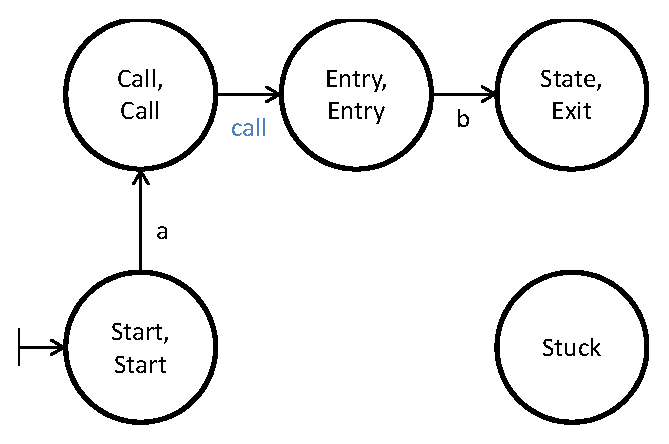
\includegraphics[width=8cm]{Figures/Figure6.eps}
  \caption{The NWA resulting from the intersection of the NWA in Figure \ref{Fig:Example1} and the NWA in Figure \ref{Fig:Intersect1}.}
  \label{Fig:Intersect2}
\end{figure}

To construct the intersection of two NWAs, the \texttt{stateIntersect} and \texttt{transitionIntersect} methods may need to be overridden to specify which states and symbols are to be considered equivalent.  The default behavior of \texttt{stateIntersect} is that any two states can be intersected, the resulting state to add to the NWA is labeled with a \texttt{Key} that is uniquely generated from the pair of the \texttt{Keys} of the two states under consideration, and the client information associated with the resulting state is \texttt{null}.  The default behavior of \texttt{transitionIntersect} is that two transitions are intersectable if the symbols that label the transitions are not \texttt{epsilon} (\texttt{$\epsilon$}) and either the symbols are the same or at least one of the symbols is a \texttt{wild} (\texttt{*}). Client information is generated through the use of the helper method \texttt{stateIntersect}, but can be altered through the use of the helper methods \texttt{intersectClientInfoInternal}, \texttt{intersectClientInfoCall}, and  \texttt{intersectClientInfoReturn}, which are invoked by \texttt{intersect} as transitions of the three different kinds involving the associated state are added.  The default behavior of \texttt{intersectClientInfoInternal}, \texttt{intersectClientInfoCall}, and \texttt{intersectClientInfoReturn} is to perform no changes to the \texttt{ClientInfo}.  These methods can be overridden to specify alternative behaviors. As intersection is performed, and the transitions of the component NWAs are traversed, \texttt{transitionIntersect} is called to determine whether a transition should be added to the result NWA.  If so, \texttt{stateIntersect} is called to determine whether the target states of the transitions in question can be joined.  Finally, if a transition is going to be added to the result NWA, \texttt{intersectClientInfoInternal}, \texttt{intersectClientInfoCall}, or \texttt{intersectClientInfoReturn} is called (depending on the type of transition) to update the \texttt{ClientInfo} associated with the target state of the transition to be added. \\

\noindent The following operations are methods of class NWA:

\begin{description}

  \item\texttt{bool stateIntersect( ref\_ptr<NWA> first, Key state1,\\ \hspace*{3.25cm} ref\_ptr<NWA> second,Key state2,\\ \hspace*{3.25cm} Key\& resSt, ref\_ptr<ClientInfo>\& resCI )}

    Determines whether the given states are considered to be equivalent for the purposes of intersection and, if so, creates the combined state, together with the client information that should be associated with the combined state and returns true.  Otherwise, returns false.
    
  \item\texttt{bool transitionIntersect( ref\_ptr<NWA> first, Key sym1,\\ \hspace*{3.25cm} ref\_ptr<NWA> second, Key sym2,\\ \hspace*{3.25cm} Key\& resSym )}

    Determines whether the given symbols are considered to be equivalent for the purposes of intersection and, if so, computes the symbol which should be associated with the combined transition and returns true.  Otherwise, returns false. 

  \item\texttt{void intersectClientInfoInternal( \\ \hspace*{3.25cm} ref\_ptr<NWA> first, Key src1, Key tgt1,\\ \hspace*{3.25cm} ref\_ptr<NWA> second, Key src2, Key tgt2,\\ \hspace*{3.25cm} Key resSym, Key resSt )}

    Alters the client information associated with \texttt{resSt} given the sources and targets (as well as access to the client information associated with each state) of the two internal transitions that are being intersected.

  \item\texttt{void intersectClientInfoCall( \\ \hspace*{3.25cm} ref\_ptr<NWA> first ,Key call1, Key entry1,\\ \hspace*{3.25cm} ref\_ptr<NWA> second, Key call2, Key entry2,\\ \hspace*{3.25cm} Key resSym, Key resSt )}

    Alters the client information associated with \texttt{resSt} given the call sites and entry points (as well as access to the client information associated with each state) of the two call transitions that are being intersected.

  \item\texttt{void intersectClientInfoReturn( \\ \hspace*{2.25cm} ref\_ptr<NWA> first, Key exit1, Key call1, Key ret1,\\ \hspace*{2.5cm} ref\_ptr<NWA> second, Key exit2, Key call2, Key ret2,\\ \hspace*{2.25cm} Key resSym, Key resSt )}

    Alters the client information assoicated with \texttt{resSt} given the exit point, call site, and return site (as well as access to the client information associated with each state) of the two return transitions that are being intersected. \\

\end{description}


Consider the slightly more complex example of computing the intersection of the NWAs shown in Figure \ref{Fig:Intersect3}.  The resulting NWA is shown in Figure \ref{Fig:Intersect4}.  Note that a state is only made final if both of its component states were final in their respective NWAs (this can be seen in the state 'Call\_1,Dead\_End' where 'Dead\_End' was final, but 'Call\_1' was not).  

\begin{figure}[htbp]
  \centering
    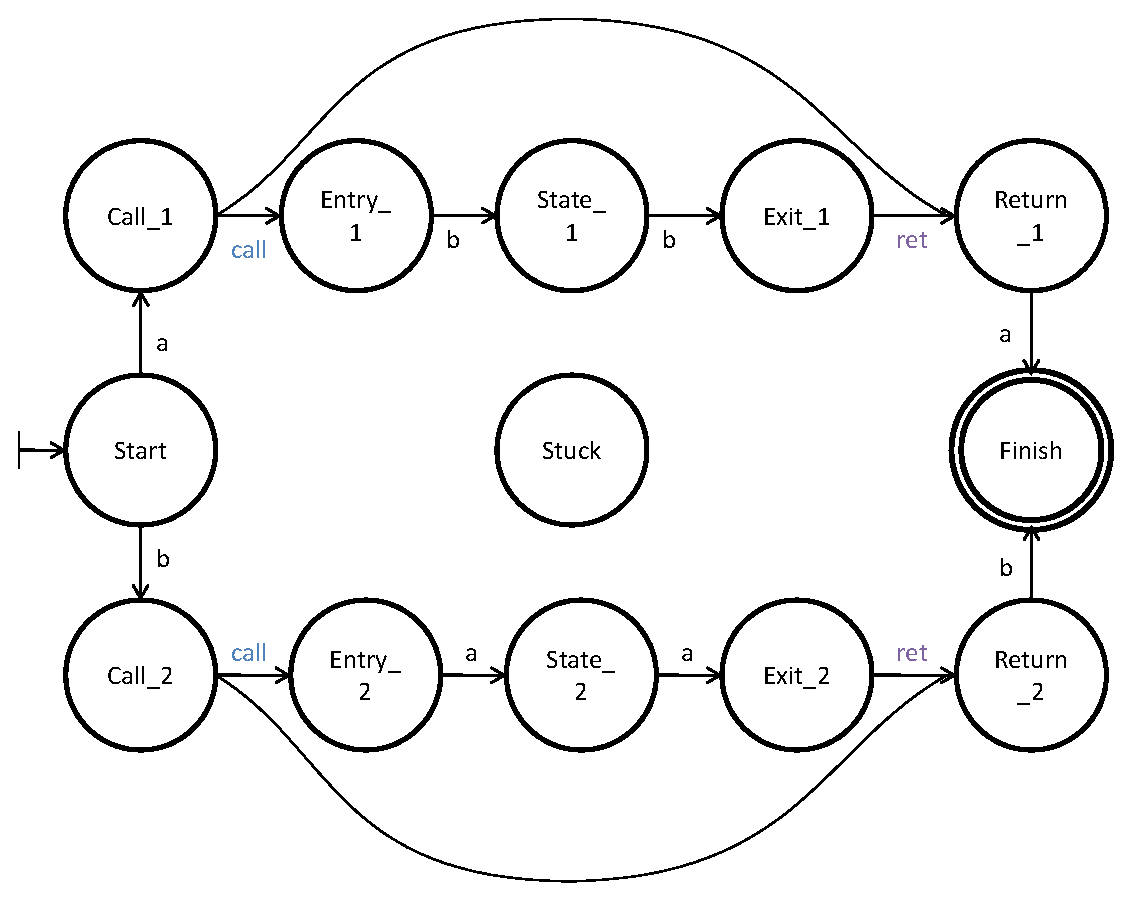
\includegraphics[width=12cm]{Figures/Figure7a.eps}
    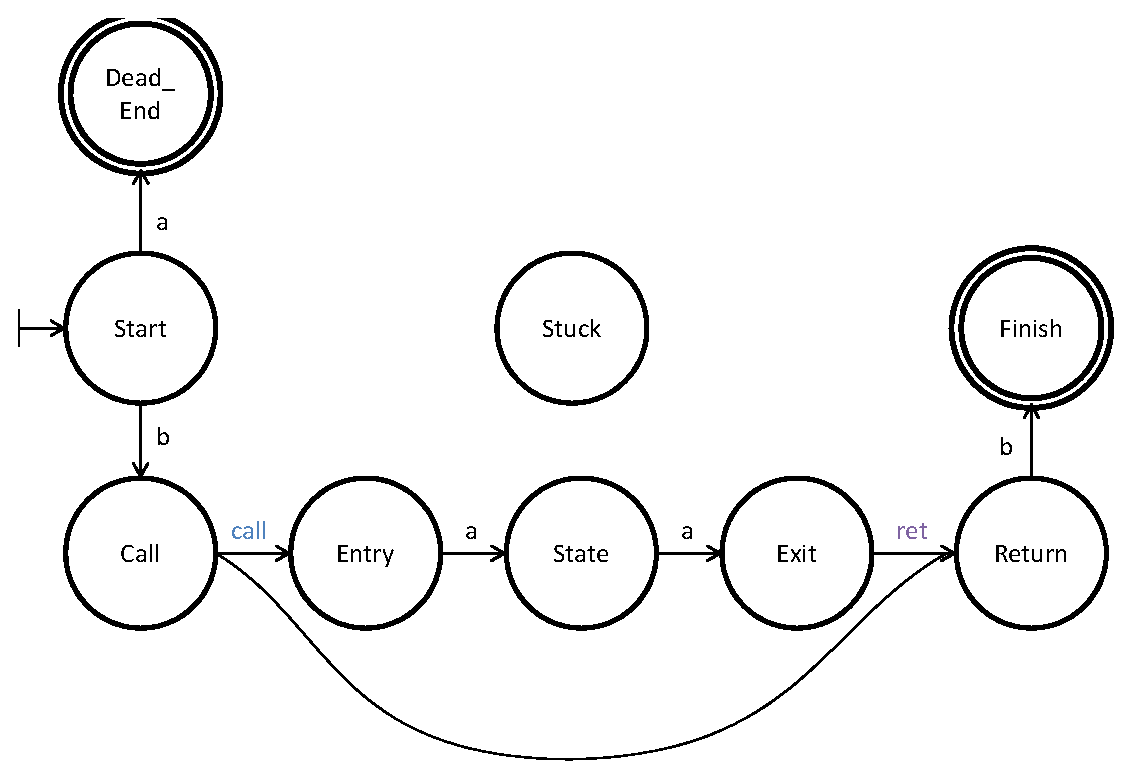
\includegraphics[width=12cm]{Figures/Figure7b.eps}
  \caption{Complex NWAs to intersect.}
  \label{Fig:Intersect3}
\end{figure}

\begin{figure}[htbp]
  \centering
    \includegraphics[width=12cm]{Figures/Figure8.eps}
  \caption{The NWA resulting from the intersection of the NWAs in Figure \ref{Fig:Intersect3}.}
  \label{Fig:Intersect4}
\end{figure}

\subsection{Concatenation}
\label{Se:Concatenation}

Consider an example of computing the concatenation of two NWAs, the NWA shown in Figure \ref{Fig:Example1} and the NWA shown in Figure \ref{Fig:Concat1}.  The concatenation is constructed by combining all states and transitions of the first NWA (shown in Figure \ref{Fig:Example1}) and all states and transitions of the second NWA (shown in Figure \ref{Fig:Concat1}) then adding internal epsilon transitions from each final state of the first NWA to each initial state of the second NWA.  In the resulting NWA, the initial states are the initial states from the first NWA; the final states are the final states of the second NWA.  If the component NWAs are  $(Q_1, \Sigma_1, {Q_0}_1, \delta_1, {Q_f}_1)$ and $(Q_2, \Sigma_2, {Q_0}_2, \delta_2, {Q_f}_2)$, then the resulting NWA is $(Q, \Sigma, Q_0, \delta, Q_f)$ where $Q = Q_1 \cup Q_2$, $\Sigma = \Sigma_1 \cup \Sigma_2$, $Q_0 = {Q_0}_1$, $\delta = \delta_1 \cup \delta_2 \cup \delta_\epsilon$ (where $\delta_\epsilon = {(q,\epsilon,q') | q \in {Q_f}_1, q' \in {Q_0}_2}$, and $Q_f = {Q_f}_2$ .  The NWA resulting from the concatenation of the NWA in Figure \ref{Fig:Example1} and the NWA shown in Figure \ref{Fig:Concat1} is shown in Figure \ref{Fig:Concat2}.

\begin{figure}[htbp]
  \centering
    \includegraphics[width=10cm]{Figures/Figure9.eps}
  \caption{Simple NWA to concatenate onto the NWA in Figure \ref{Fig:Example1}.}
  \label{Fig:Concat1}
\end{figure}

\begin{figure}[htbp]
  \centering
    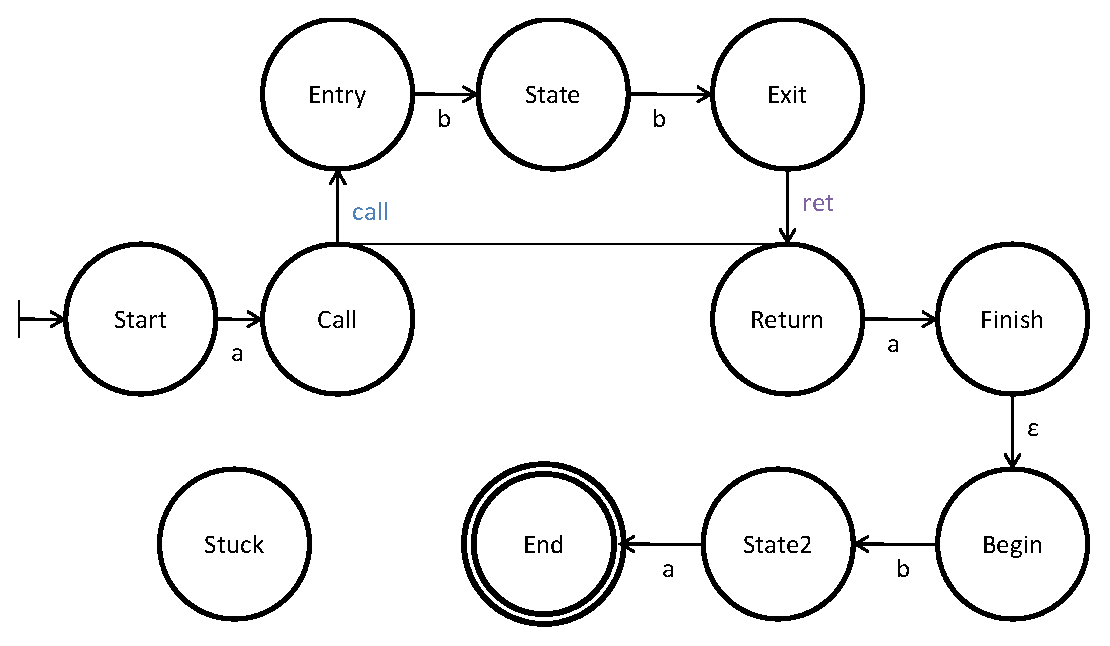
\includegraphics[width=12cm]{Figures/Figure10.eps}
  \caption{The NWA resulting from the concatenation of the NWA in Figure \ref{Fig:Example1} with the NWA in Figure \ref{Fig:Concat1}.}
  \label{Fig:Concat2}
\end{figure}

The stuck state of the NWA on which the concat method is called cannot be any state (except the stuck state) in either of the component NWAs.  Furthermore, in order to construct the concatenation of two NWAs, the state sets of the NWAs cannot overlap, i.e. $Q_1 \cap Q_2 = \emptyset$. Client information is copied directly from the component NWAs using the \texttt{ClientInfo} copy constructor.

\subsection{Kleene-Star}
\label{Se:Star}

Consider an example of computing the Kleene-Star of the NWA shown in Figure \ref{Fig:Star1}.  If the component NWA is $(Q, \Sigma, Q_0, \delta, Q_f)$, then the result of performing Kleene-Star on that NWA is $(Q \cup Q', \Sigma, Q_0', \delta', Q_0')$ where $Q' = \{q' | q \in Q\}$ and $\delta' = \{\delta_i',\delta_c',\delta_r'\}$ such that 

\begin{enumerate} 

\item For all $(q,a,p) \in \delta_i$, the result NWA has $(q,a,p) \in \delta_i'$ and $(q',a,p') \in \delta_i'$, and if $p \in Q_f$, then $(q,a,r') \in \delta_i'$ and $(q',a,r') \in \delta_i'$ for each $r \in Q_0$, 

\item For all $(q,a,p) \in \delta_c$, the result NWA has $(q,a,p) \in \delta_c'$ and $(q',a,p) \in \delta_c'$, and if $p \in Q_f$, then $(q,a,r') \in \delta_c'$ and $(q',a,r') \in \delta_c'$ for each $r \in Q_0$, 

\item For all $(q,r,a,p) \in \delta_r$, the result NWA has $(q,r,a,p) \in \delta_r'$ and $(q,r',a,p') \in \delta_r'$, and if $p \in Q_f$, then $(q,r,a,s') \in \delta_r'$ and $(q,r',a,s') \in \delta_r'$ for each $s \in Q_0$, and 

\item For all $(q,r,a,p) \in \delta_r$ with $r \in Q_0$, the result NWA has $(q',s,a,p') \in \delta_r'$ for each $s \in Q \cup Q'$, and if $p \in Q_f$, then $(q',s,a,t') \in \delta_r'$ for each $s \in Q \cup Q'$ and $t \in Q_0$

\end{enumerate}  

\noindent The NWA resulting from performing Kleene-Star on the NWA shown in Figure \ref{Fig:Star1} is shown in Figure \ref{Fig:Star2}.

\begin{figure}[htbp]
  \centering
    \includegraphics[width=10cm]{Figures/Figure11.eps}
  \caption{An NWA on which to perform Kleene-Star.}
  \label{Fig:Star1}
\end{figure}

\begin{figure}[htbp]
  \centering
    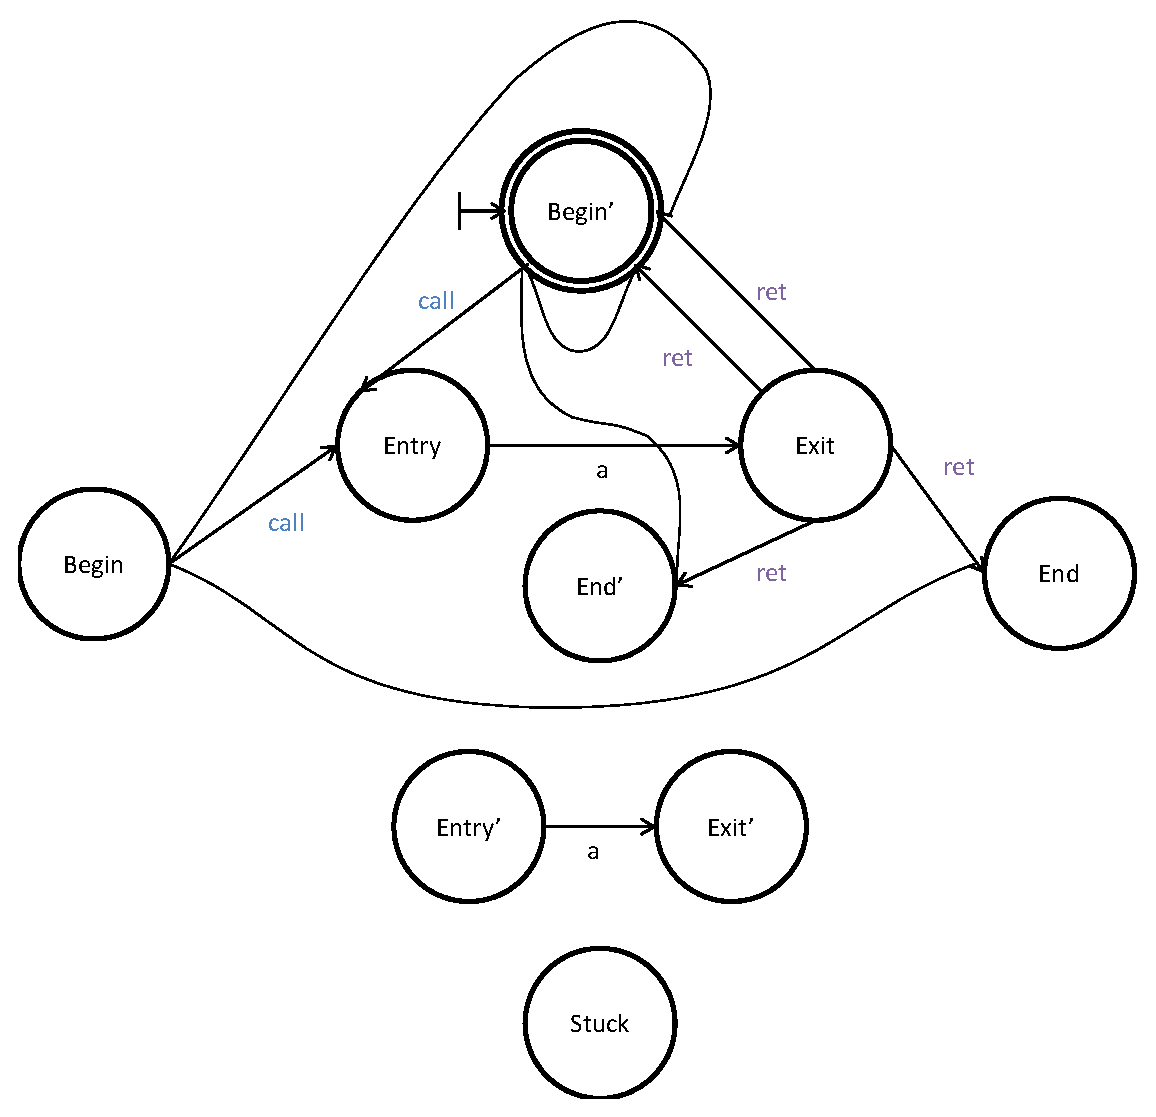
\includegraphics[width=12cm]{Figures/Figure12.eps}
  \caption{The NWA resulting from performing Kleene-Star on the NWA in Figure \ref{Fig:Star1}.}
  \label{Fig:Star2}
\end{figure}

The stuck state of the NWA on which the Kleene-Star method is called cannot be any state in the component NWA or the primed version of any such state (i.e., $stuck \not\in Q \cup Q'$) unless it is the stuck state.  Client information is copied directly from the component NWA (using the \texttt{ClientInfo} copy constructor) such that for each $q \in Q$, $q$ and $q'$ have the same client information.   

%Consider the slightly more complex example of computing the Kleene-Star of the NWA shown in Figure \ref{Fig:Star3}.  The resulting NWA is shown in Figure \ref{Fig:Star4}.

%\begin{figure}[htbp]
%  \centering
%    \includegraphics[angle=270,width=10cm]{Figures/Figure13.pdf}
%  \caption{Complex NWA on which to perform Kleene-Star.}
%  \label{Fig:Star3}
%\end{figure}

%\begin{figure}[htbp]
%  \centering
%    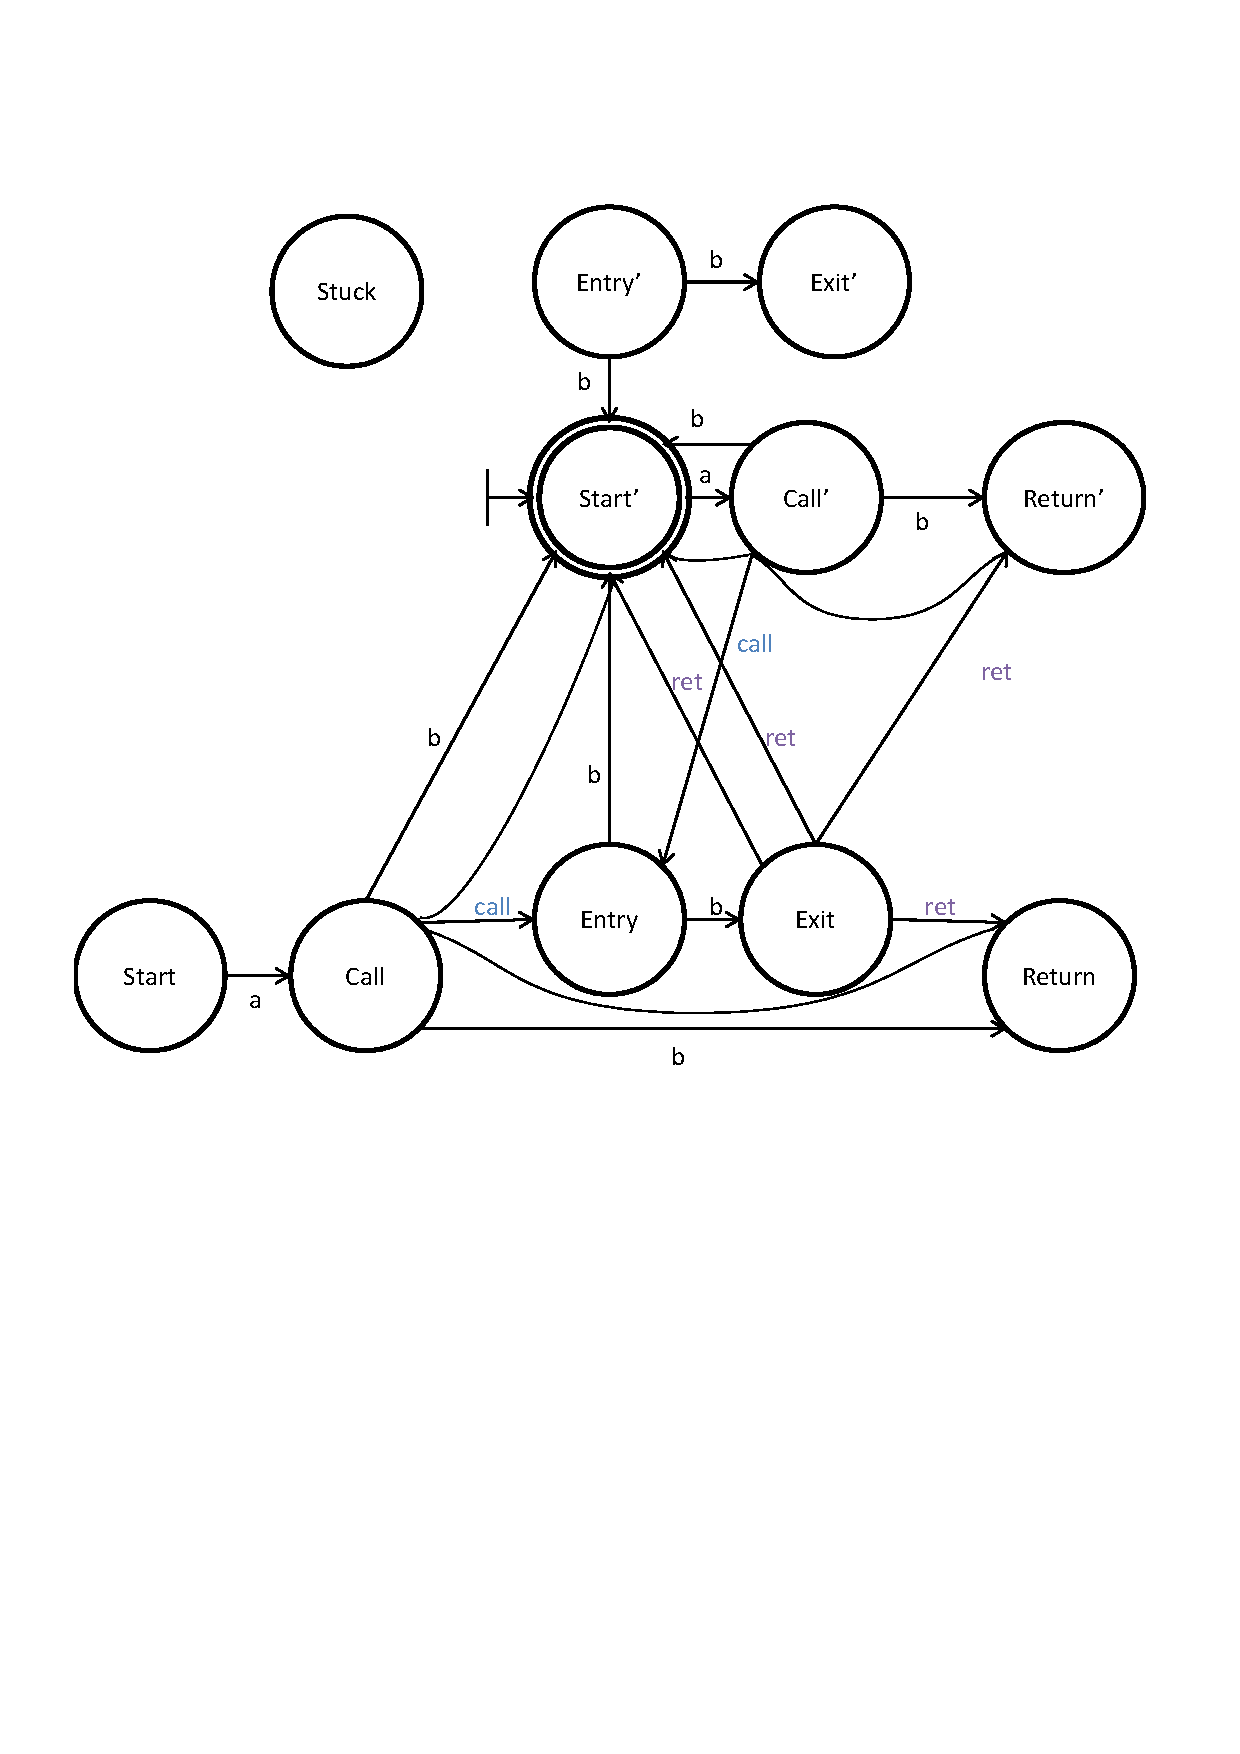
\includegraphics[angle=270,width=12cm]{Figures/Figure14.pdf}
%  \caption{The NWA resulting from performing Kleene-Star on the NWA in Figure \ref{Fig:Star3}.}
%  \label{Fig:Star4}
%\end{figure}

\subsection{Reverse}
\label{Se:Reverse}

Consider an example of computing the reverse of the NWA shown in Figure \ref{Fig:Example1}.  If the component NWA is $(Q, \Sigma, Q_0, \delta, Q_f)$, then the result of reversing that NWA is $(Q, \Sigma, Q_0, \delta_{rev}, Q_f)$ such that

\begin{enumerate}

\item For all $(q,\sigma,q') \in \delta_i$, the result NWA has $(q',\sigma,q) \in {\delta_{rev}}_i$ 

\item For all $(q_c,\sigma,q_e) \in \delta_c$, the result NWA has $(q_e,\sigma,q_c) \in {\delta_{rev}}_c$

\item For all $(q_x,q_c,\sigma,q_r) \in \delta_r$ and $(q_c,\sigma,q_e) \in \delta_c$ (where the $q_c$s are the same), the result NWA has $(q_r,q_e,\sigma,q_x) \in {\delta_{rev}}_r$

\end{enumerate}

\noindent The NWA resulting from performing reverse on the NWA shown in Figure \ref{Fig:Example1} is shown in Figure \ref{Fig:Reverse1}.
 
\begin{figure}[htbp]
  \centering
    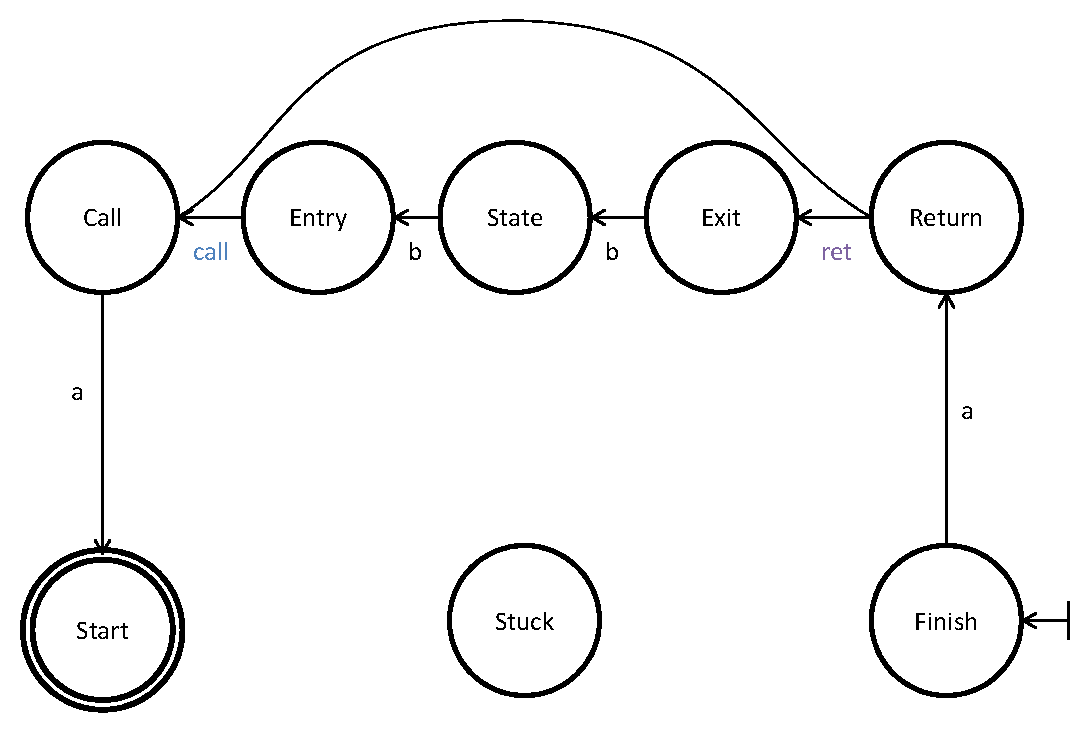
\includegraphics[width=12cm]{Figures/Figure15.eps}
  \caption{The NWA resulting from performing reverse on the NWA in Figure \ref{Fig:Example1}.}
  \label{Fig:Reverse1}
\end{figure}

The stuck state of the NWA on which the reverse method is called cannot be any state in the component NWA (including the stuck state).  Client information is copied directly from the component NWA using the \texttt{ClientInfo} copy constructor.

\subsection{Determinize}
\label{Se:Determinize}

\begin{definition}
An NWA, $(Q,\Sigma,Q_0,\delta,Q_f)$, is \textbf{deterministic} if 

\begin{enumerate} 

\item $|Q_0| = 1$, 

\item 
 For all $q \in Q$, if $(q,*,q') \in \delta_i$ then $|\{q'|(q,\sigma,q') \in \delta_i\}| = 0$; otherwise for all $\sigma \in \Sigma - \{*\} |\{q'|(q,\sigma,q') \in \delta_i\}| = 1$,

 for all $q \in Q$, if $(q,*,q') \in \delta_c$ then $ |\{q'|(q,\sigma,q') \in \delta_c\}| = 0$; otherwise for all $\sigma \in \Sigma - \{*\} |\{q'|(q,\sigma,q') \in \delta_c\}| = 1$,  and

 for all $q,q' \in Q$, if $(q,q',*,q'') \in \delta_r$ then $|\{q''|(q,q',\sigma,q'') \in \delta_r\}| = 0$; otherwise for all $\sigma \in \Sigma - \{*\} |\{q''|(q,q',\sigma,q'') \in \delta_r\}| = 1$, and

\item For all $(q,\sigma,q') \in \delta_i, \sigma \neq \epsilon$,

 for all $(q,\sigma,q') \in \delta_c, \sigma \neq \epsilon$,  and 

 for all $(q,q',\sigma,q'') \in \delta_r, \sigma \neq \epsilon$.\\

\end{enumerate}

If an NWA is not deterministic, then it is \textbf{non-deterministic}.
\end{definition}

Consider an example of determinizing a simple nondeterministic NWA, the NWA shown in Figure \ref{Fig:Det1}.  The deterministic NWA is computed by a generalization of the classical subset construction.  Instead of the states in the determinized NWA being subsets of the original NWA, states of  the determinized NWA are sets of state pairs (i.e., binary relations on states).  To support determinization, the library provides class \texttt{BinaryRelation}, which is a set of \texttt{Key} pairs. \cite{DLT:AM2006}  The resulting NWA is shown in Figure \ref{Fig:Det2}.

\begin{figure}[htbp]
  \centering
    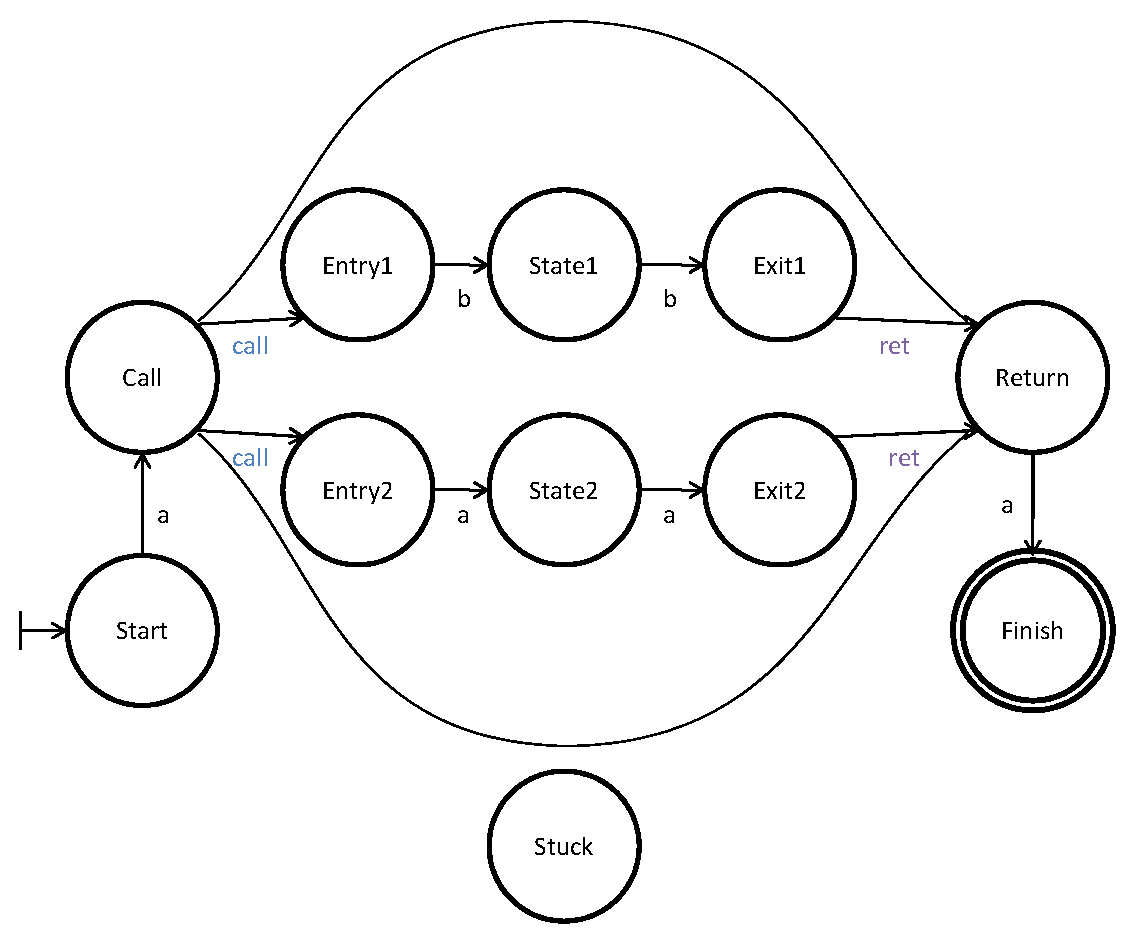
\includegraphics[width=12cm]{Figures/Figure16.eps}
  \caption{Simple nondeterministic NWA.}
  \label{Fig:Det1}
\end{figure}


\begin{figure}[htbp]
  \centering
    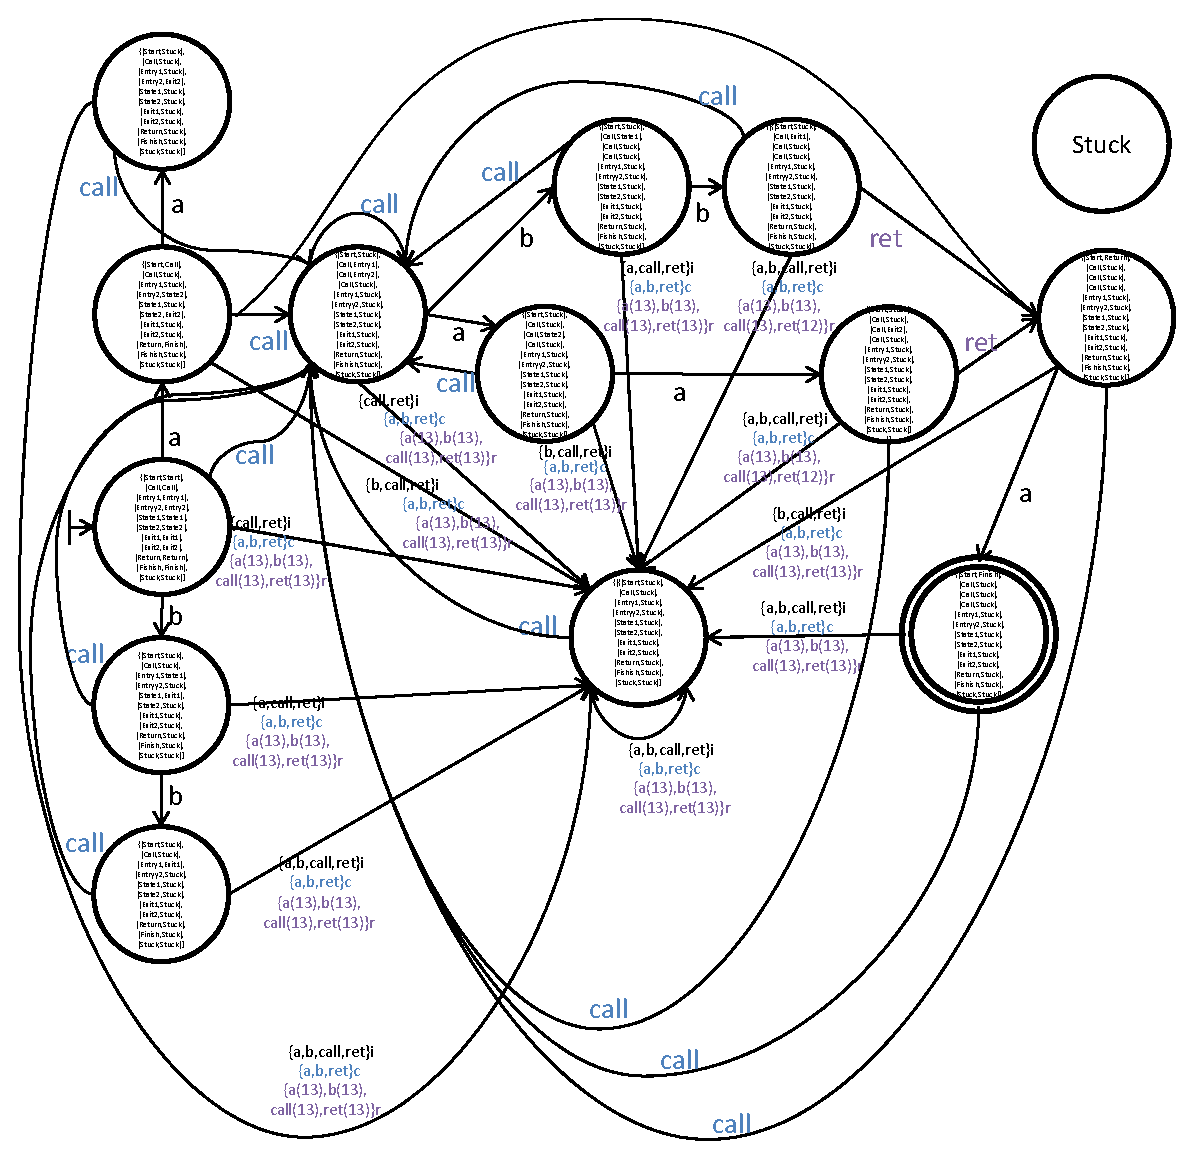
\includegraphics[width=16cm]{Figures/Figure17.eps}
  \caption{The NWA resulting from determinizing the NWA in Figure \ref{Fig:Det1}.}
  \label{Fig:Det2}
\end{figure}


Client information is generated through the use of the helper method \texttt{mergeClientInfo}, but can be altered through the use of the helper methods \texttt{mergeClientInfoInternal}, \texttt{mergeClientInfoCall}, and \texttt{mergeClientInfoReturn}, which are invoked by \texttt{determinize} as transitions of the three kinds involving the associated state are added.  The default behavior of \texttt{mergeClientInfo}, is that the \texttt{ClientInfo} associated with the resulting state is \texttt{null}.  The default behavior of \texttt{mergeClientInfoInternal}, \texttt{mergeClientInfoCall}, and \texttt{mergeClientInfoReturn} is to make no changes to the the \texttt{ClientInfo}.  These methods can be overridden to specify alternative behaviors.  As determinization is performed, \texttt{mergeClientInfo} is called each time a new state is created.  Then, as each transition is added \texttt{mergeClientInfoInternal}, \texttt{mergeClientInfoCall}, or \texttt{mergeClientInfoReturn} is called (depending on the type of transition that is added) to update the \texttt{ClientInfo} associated with the target state of the transition to be added. \\

\noindent The following operations are methods of class NWA:

\begin{description}

  \item\texttt{void mergeClientInfo( ref\_ptr<NWA> first,\\ \hspace*{3.25cm} BinaryRelation const\& binRel,\\ \hspace*{3.25cm} St resSt, ref\_ptr<ClientInfo>\& resCI )}

    Computes the client information that should be associated with the given state.

  \item\texttt{void mergeClientInfoInternal( ref\_ptr<NWA> first,\\ \hspace*{3.25cm} BinaryRelation const\& binRelSource,\\ \hspace*{3.25cm} BinaryRelation const\& binRelTarget,\\ \hspace*{3.25cm} Key sourceSt, Key resSym, Key resSt,\\ \hspace*{3.25cm} ref\_ptr<ClientInfo>\& resCI )}

    Alters the client information associated with \texttt{resSt} given the details of the internal transition to be added to the NWA.

  \item\texttt{void mergeClientInfoCall( ref\_ptr<NWA> first,\\ \hspace*{3.25cm} BinaryRelation const\& binRelCall,\\ \hspace*{3.25cm} BinaryRelation const\& binRelEntry,\\ \hspace*{3.25cm} Key callSt, Key resSym, Key resSt,\\ \hspace*{3.25cm} ref\_ptr<ClientInfo>\& resCI )}

    Alters the client information associated with \texttt{resSt} given the details of the call transition to be added to the NWA.

  \item\texttt{void mergeClientInfoReturn( ref\_ptr<NWA> first,\\ \hspace*{3.25cm} BinaryRelation const\& binRelExit,\\ \hspace*{3.25cm} BinaryRelation const\& binRelCall,\\ \hspace*{3.25cm} BinaryRelation const\& binRelReturn,\\ \hspace*{3.25cm} Key exitSt, Key callSt, Key resSym,\\ \hspace*{3.25cm} Key resSt, ref\_ptr<ClientInfo>\& resCI )}

    Alters the client information associated with \texttt{resSt} given the details of the return transition to be added to the NWA. \\

\end{description}

%Consider the slightly more complex determinization of the NWA shown in Figure \ref{Fig:Det3}.  The resulting NWA is shown in Figure \ref{Fig:Det4}.

%\begin{figure}[htbp]
%  \centering
%    \includegraphics[angle=270,width=12cm]{Figures/Figure18.pdf}
%  \caption{Complex nondeterministic NWA.}
%  \label{Fig:Det3}
%\end{figure}

%\begin{figure}[htbp]
%  \centering
%    \includegraphics[angle=270,width=12cm]{Figures/Figure19.pdf}
%  \caption{The NWA resulting from determinizing the NWA in Figure \ref{Fig:Det3}.}
%  \label{Fig:Det4}
%\end{figure}

\subsection{Complement}
\label{Se:Complement}

Consider an example of computing the complement of the simple NWA shown in Figure \ref{Fig:Det1}.  The complement is performed by first determinizing the NWA and then complementing the final state set of the determinized NWA.  The NWA resulting from performing the complement of the NWA shown in Figure \ref{Fig:Det1} is shown in Figure \ref{Fig:Comp1}.

\begin{figure}[htbp]
  \centering
    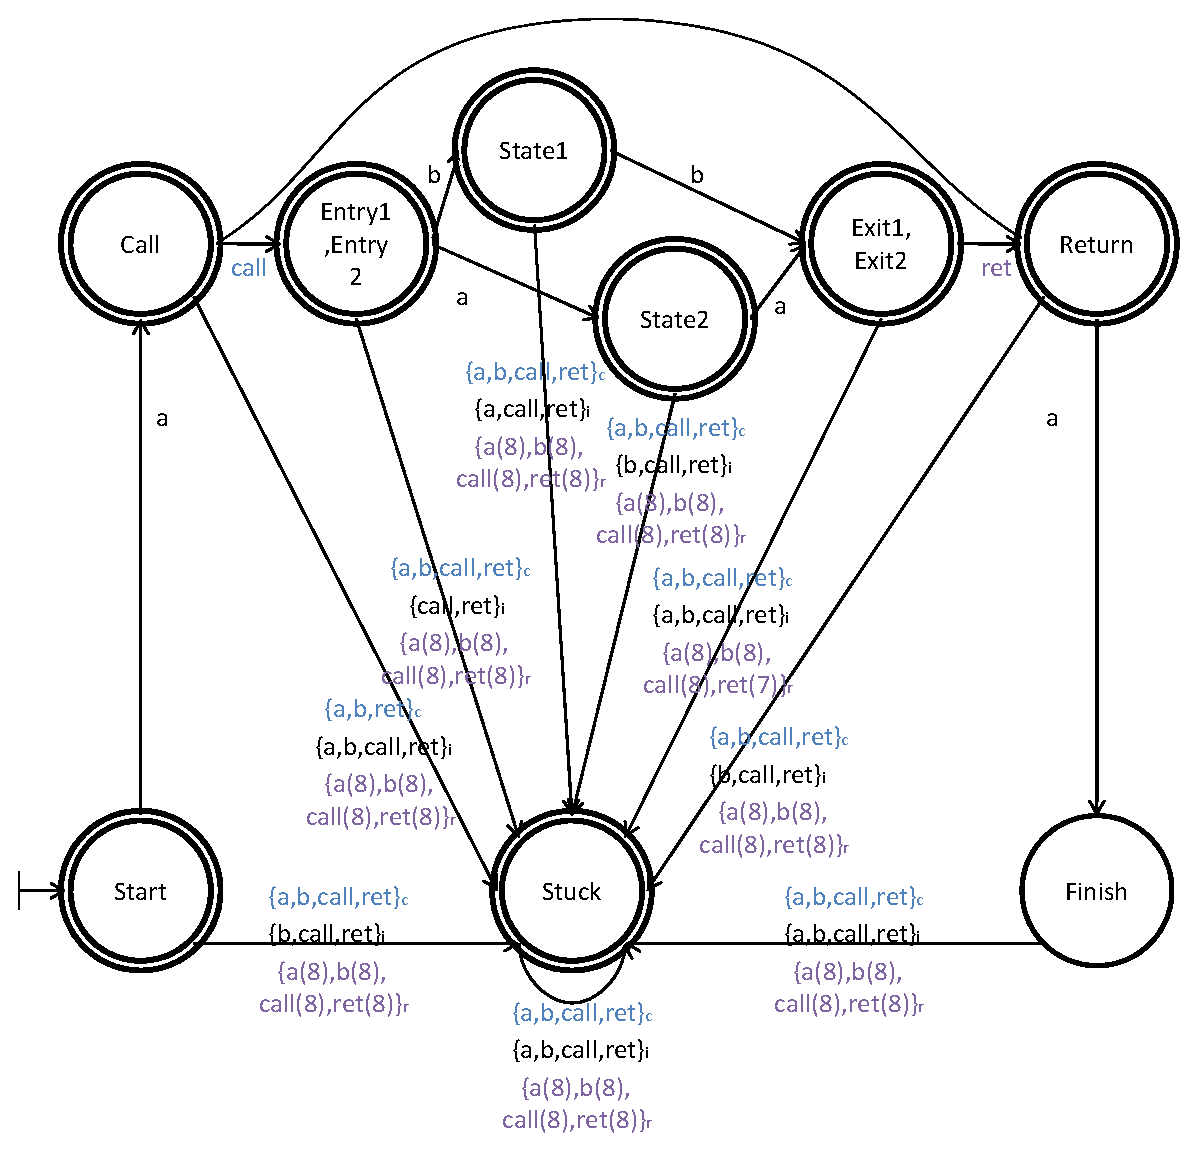
\includegraphics[width=12cm]{Figures/Figure20.eps}
  \caption{The complement of the NWA in Figure \ref{Fig:Det1} (the determinization of which is shown in Figure \ref{Fig:Det2}).}
  \label{Fig:Comp1}
\end{figure}

Because all non-final states (including the stuck state) become final states in the process of complementation, all implicit transitions are materialized and the resulting NWA is an NWA of type 2.  Client information is copied directly from the determinization of the component NWA using the \texttt{ClientInfo} copy constructor.

\section{Conversions}
\label{Se:Conversions}


An NWA can both be constructed from a WALi WPDS and used to construct a WALi WPDS.  \textbf{However, the construction of an NWA from a WPDS is not the inverse of constructing a WPDS from an NWA, i.e., one cannot perform the two conversions in sequence and obtain the identity conversion.} \\

\noindent The following operations are methods of class NWA:

\begin{description}

  \item\texttt{WPDS plusWPDS( const WPDS\& base )}

    This operation is an NWA method.  It returns the WPDS that is the product of the NWA referred to by \texttt{this} and the given WPDS. \cite{advancedquerying}

  \item\texttt{void PDStoNWA( const WPDS\& pds )}

    This operation is an NWA method; the NWA referred to by \texttt{this} is converted to the NWA that is equivalent to the given PDS.  This method should not be called on an NWA of type 2, otherwise there is an assertion violation.  Typical sequence of operations: construct A; A.PDSto NWA(pds);

  \item\texttt{static ref\_ptr<NWA> PDStoNWA( const WPDS\& pds, Key stuck )}

    Constructs and returns the NWA that is equivalent to the given PDS, having the stuck state \texttt{stuck}.

  \item\texttt{WPDS NWAtoPDScalls( WeightGen<Client>\& wg ) const}

    This operation is an NWA method.  It constructs the WPDS that keeps call states on the stack that is equivalent to the NWA referred to by \texttt{this}.  It uses \texttt{wg} to determine weights for WPDS rules (see Section \ref{Se:NWAtoPDS}).

  \item\texttt{WPDS NWAtoBackwardsPDScalls( WeightGen<Client>\& wg ) const}

    This operation is an NWA method.  It constructs the backwards WPDS that keeps call states on the stack that is equivalent to the NWA referred to by \texttt{this}.  It uses \texttt{wg} to determine weights for WPDS rules (see Section \ref{Se:NWAtoPDS}).

  \item\texttt{WPDS NWAtoPDSreturns( WeightGen<Client>\& wg ) const}

    This operation is an NWA method.  It constructs the WPDS that keeps return states on the stack thatis equivalent to the NWA referred to by \texttt{this}.  It uses \texttt{wg} to determine weights for WPDS rules (see Section \ref{Se:NWAtoPDS}).  (Deprecated)

  \item\texttt{WPDS NWAtoBackwardsPDSreturns( WeightGen<Client>\& wg ) const}

    This operation is an NWA method.  It constructs the backwards WPDS that keeps return states on the stack that is equivalent to the NWA referred to by \texttt{this}.  It uses \texttt{wg} to determine weights for WPDS rules (see Section \ref{Se:NWAtoPDS}).  (Deprecated) \\

\end{description}

\subsection{PDS to NWA}
\label{Se:PDStoNWA}

The last way to build an NWA is to convert a PDS into an NWA.  Consider, as an example, converting the PDS in Figure \ref{Fig:PDStoNWA1} into an NWA.  The conversion is performed by:

\begin{enumerate}

\item Adding $( (p,q), q, (p',q') )$ to $\delta_i$ of the NWA for each $\langle p,q \rangle \hookrightarrow \langle p',q' \rangle \in \Delta_1$ in the PDS

\item Adding $( (p,q_c), q_c, (p',q_e) )$ to $\delta_c$ of the NWA for each $\langle p,q_c \rangle \hookrightarrow \langle p',q_e \hspace{.1cm} q_r \rangle \in \Delta_2$ in the PDS

\item Adding $( (p'',q_x), (p,q_c), q_x, (p''',q_r) )$ to $\delta_r$ of the NWA for all $(q_c,q_r)$ pairs such that $\langle p,q_c \rangle \hookrightarrow \langle p',q_e \hspace{.1cm} q_r \rangle \in \Delta_2$ for each $\langle p'',q_x \rangle \hookrightarrow \langle p''',\epsilon \rangle \in \Delta_0$ in the PDS

\end{enumerate}

\begin{figure}[htbp]
  \centering
    \begin{description}
      \centering
      \item $\langle p,main \rangle \hookrightarrow \langle p,q_1 \rangle$
      \item $\langle p,q_1 \rangle \hookrightarrow \langle p,c_1 \rangle$
      \item $\langle p,c_1 \rangle \hookrightarrow \langle p,e \hspace{.1cm} r_1 \rangle$
      \item $\langle p,e \rangle \hookrightarrow \langle p,q_2 \rangle$
      \item $\langle p,q_2 \rangle \hookrightarrow \langle p,q_3 \rangle$
      \item $\langle p,q_3 \rangle \hookrightarrow \langle p,x \rangle$
      \item $\langle p,x \rangle \hookrightarrow \langle p,\epsilon \rangle$
      \item $\langle p,r_1 \rangle \hookrightarrow \langle p,q_4 \rangle$
      \item $\langle p,q_4 \rangle \hookrightarrow \langle p,q_5 \rangle$
      \item $\langle p,q_5 \rangle \hookrightarrow \langle p,c_2 \rangle$
      \item $\langle p,c_2 \rangle \hookrightarrow \langle p,e \hspace{.1cm} r_2 \rangle$
      \item $\langle p,r_2 \rangle \hookrightarrow \langle p,q_6 \rangle$
      \item $\langle p,q_6 \rangle \hookrightarrow \langle p,exit \rangle$
    \end{description}
  \caption{An example PDS.}
  \label{Fig:PDStoNWA1}
\end{figure}

\noindent The NWA resulting from converting the PDS shown in Figure \ref{Fig:PDStoNWA1} into an NWA is shown in Figure \ref{Fig:PDStoNWA2}.

\begin{figure}[htbp]
  \centering
    \includegraphics[width=12cm]{Figures/Figure22.eps}
  \caption{The NWA resulting from converting the PDS in Figure \ref{Fig:PDStoNWA1} into an NWA.}
  \label{Fig:PDStoNWA2}
\end{figure}

The client information for all states in the resulting NWA are set to \texttt{null}.

\subsection{NWA to PDS}
\label{Se:NWAtoPDS}

An NWA can also be converted into a WPDS.  In this way the reachability queries that are a part of the main WALi library can still be used effectively.  There are four variations on the NWA to WPDS conversion: \begin{inparaenum} \item forwards flow with call states on the stack \item backwards flow with call states on the stack \item forwards flow with return states on the stack \item backwards flow with return states on the stack. \end{inparaenum}  All four variations use \texttt{WeightGen} to determine weights for WPDS rules.

\texttt{WeightGen} provides algorithms for calculating the weights for WPDS rules.  See \cite[\S4-\S5]{wali} for details about weight domains. \\ 

\noindent The following operations are methods of class WeightGen:

\begin{description} 

  \item \texttt{sem\_elem\_t getOne()} 

    Returns an instance of the $\bar{1}$ element of the weight domain.

  \item \texttt{sem\_elem\_t getWeight( Key source, ref\_ptr<ClientInfo> sourceInfo, \\  
                              \hspace*{3.25cm} Key symbol, Kind k, \\
                              \hspace*{3.25cm} Key target, ref\_ptr<ClientInfo> targetInfo )} 

    Computes and returns the weight (in the desired semiring) for a WPDS rule from the (\texttt{kind}) transition between \texttt{source} and \texttt{target} labeled with symbol \texttt{symbol}.

  \item \texttt{sem\_elem\_t getWildWeight( \\
                              \hspace*{3.25cm} Key source, ref\_ptr<ClientInfo> sourceInfo, \\
                              \hspace*{3.25cm} Key target, ref\_ptr<ClientInfo> targetInfo )}. 

    Computes and returns the weight (in the desired semiring) for a WPDS rule from the transition between \texttt{source} and \texttt{target} labeled with the meta-symbol \texttt{*}. \\

\end{description}


\noindent \textbf{1. Forwards Flow Stacking Calls} \\

\noindent Consider, as an example, converting the NWA in Figure \ref{Fig:NWAtoPDS5} into a WPDS.  The conversion is performed by:

\begin{enumerate}

\item For each $(q,\sigma,q')$ $\in \delta_i$ in the NWA, adding $\langle p,q \rangle \hookrightarrow \langle p,q' \rangle$ to $\Delta_1$ of the WPDS (with weight \texttt{wg.getWeight($q$,$CI_q$,$\sigma$,INTRA,$q'$,$CI_{q'}$}) or \texttt{wg.getWildWeight($q$,$CI_q$,$q'$,$CI_{q'}$)} depending on $\sigma$).

\item For each $(q_c,\sigma, q_e)$ $\in \delta_c$ in the NWA, adding $\langle p,q_c \rangle \hookrightarrow \langle p, q_e \hspace{.1cm} q_c \rangle$ to $\Delta_2$ of the WPDS (with weight \texttt{wg.getWeight($q_c$,$CI_{q_c}$,$\sigma$,CALL\_TO\_ENTRY,$q_e$,$CI_{q_e}$)} or \texttt{wg.getWildWeight($q_c$,$CI_{q_c}$,$q_e$,$CI_{q_e}$)} depending on $\sigma$).

\item For each $(q_x,q_c,\sigma,q_r)$ $\in \delta_r$ in the NWA, adding $\langle p,q_x \rangle \hookrightarrow \langle p_{q_x},\epsilon \rangle$ to $\Delta_0$ of the WPDS (with weight \texttt{wg.getWeight($q_x$,$CI_{q_x}$,$\sigma$,EXIT\_TO\_RET,$q_r$,$CI_{q_r}$)} or \texttt{wg.getWildWeight($q_x$,$CI_{q_x}$,$q_r$,$CI_{q_r}$)} depending on $\sigma$) and $\langle p_{q_x},q_c \rangle \hookrightarrow \langle p,q_r \rangle$ to $\Delta_1$ of the WPDS (with weight \texttt{wg.getOne()}).

\end{enumerate}

\noindent The WPDS resulting from converting the PDS shown in Figure \ref{Fig:NWAtoPDS1} into a WPDS is shown in Figure \ref{Fig:NWAtoPDS4}. \\

\begin{figure}[htbp]
  \centering
    \begin{description}
      \centering
      \item $\langle p,main \rangle \hookrightarrow \langle p,q_1 \rangle$
      \item $\langle p,q_1 \rangle \hookrightarrow \langle p,c_1 \rangle$
      \item $\langle p,e \rangle \hookrightarrow \langle p,q_2 \rangle$
      \item $\langle p,q_2 \rangle \hookrightarrow \langle p,q_3 \rangle$
      \item $\langle p,q_3 \rangle \hookrightarrow \langle p,x \rangle$
      \item $\langle p,r_1 \rangle \hookrightarrow \langle p,q_4 \rangle$
      \item $\langle p,q_4 \rangle \hookrightarrow \langle p,q_5 \rangle$
      \item $\langle p,q_5 \rangle \hookrightarrow \langle p,c_2 \rangle$
      \item $\langle p,r_2 \rangle \hookrightarrow \langle p,q_6 \rangle$
      \item $\langle p,q_6 \rangle \hookrightarrow \langle p,exit \rangle$
      \item $\langle p,c_1 \rangle \hookrightarrow \langle p,e \hspace{.1cm} c_1 \rangle$
      \item $\langle p,c_2 \rangle \hookrightarrow \langle p,e \hspace{.1cm} c_2 \rangle$
      \item $\langle p,x \rangle \hookrightarrow \langle p_x, \epsilon \rangle$
      \item $\langle p_x,c_1 \rangle \hookrightarrow \langle p,r_1 \rangle$
      \item $\langle p,x \rangle \hookrightarrow \langle p_x, \epsilon \rangle$
      \item $\langle p_x,c_2 \rangle \hookrightarrow \langle p,r_2 \rangle$
    \end{description}
  \caption{The PDS resulting from converting the NWA shown in Figure \ref{Fig:NWAtoPDS1} into a PDS.}
  \label{Fig:NWAtoPDS4}
\end{figure}

\noindent \textbf{2. Backwards Flow Stacking Calls} \\

\noindent Consider, as an example, converting the NWA in Figure \ref{Fig:NWAtoPDS1} into a backwards flow WPDS.  The conversion is performed by:

\begin{enumerate}

\item For each $(q,\sigma,q')$ $\in \delta_i$ in the NWA, adding $\langle p,q' \rangle \hookrightarrow \langle p,q \rangle$ to $\Delta_1$ of the WPDS (with weight \texttt{wg.getWeight($q$,$CI_q$,$\sigma$,INTRA,$q'$,$CI_{q'}$}) or \texttt{wg.getWildWeight($q$,$CI_q$,$q'$,$CI_{q'}$)} depending on $\sigma$).

\item For each $(q_c,\sigma, q_e)$ $\in \delta_c$ and $(q_x,q_c,\gamma,q_r)$ $\in \delta_r$ in the NWA, adding $\langle p,q_e \rangle \hookrightarrow \langle p_{q_e},\epsilon \rangle$ to $\Delta_0$ of the WPDS (with weight \texttt{wg.getWeight($q_c$,$CI_{q_c}$,$\sigma$,CALL\_TO\_ENTRY,$q_e$,$CI_{q_e}$)} or \texttt{wg.getWildWeight($q_c$,$CI_{q_c}$,$q_e$,$CI_{q_e}$)} depending on $\sigma$) and $\langle p_{q_e},q_r \rangle \hookrightarrow \langle p,q_c \rangle$ to $\Delta_1$ of the WPDS (with weight \texttt{wg.getOne()} ).

\item For each $(q_x,q_c,\sigma,q_r) \in \delta_r$ in the NWA, adding $\langle p,q_r \rangle \hookrightarrow \langle p,q_x \hspace{.1cm} q_r \rangle$ to $\Delta_2$ of the WPDS (with weight \texttt{wg.getWeight($q_x$,$CI_{q_x}$,$\sigma$,EXIT\_TO\_RET,$q_r$,$CI_{q_r}$)} or \texttt{wg.getWildWeight($q_x$,$CI_{q_x}$,$q_r$,$CI_{q_r}$)} depending on $\sigma$).

\end{enumerate}

\noindent The WPDS resulting from converting the PDS shown in Figure \ref{Fig:NWAtoPDS1} into a backwards flow WPDS is shown in Figure \ref{Fig:NWAtoPDS5}. \\

\begin{figure}[htbp]
  \centering
    \begin{description}
      \centering
      \item $\langle p,q_1 \rangle \hookrightarrow \langle p,main \rangle$
      \item $\langle p,c_1 \rangle \hookrightarrow \langle p,q_1 \rangle$
      \item $\langle p,q_2 \rangle \hookrightarrow \langle p,e \rangle$
      \item $\langle p,q_3 \rangle \hookrightarrow \langle p,q_2 \rangle$
      \item $\langle p,x \rangle \hookrightarrow \langle p,q_3 \rangle$
      \item $\langle p,q_4 \rangle \hookrightarrow \langle p,r_1 \rangle$
      \item $\langle p,q_5 \rangle \hookrightarrow \langle p,q_4 \rangle$
      \item $\langle p,c_2 \rangle \hookrightarrow \langle p,q_5 \rangle$
      \item $\langle p,q_6 \rangle \hookrightarrow \langle p,r_2 \rangle$
      \item $\langle p,exit \rangle \hookrightarrow \langle p,q_6 \rangle$
      \item $\langle p,r_1 \rangle \hookrightarrow \langle p,x \hspace{.1cm} r_1 \rangle$
      \item $\langle p,r_2 \rangle \hookrightarrow \langle p,x \hspace{.1cm} r_2 \rangle$
      \item $\langle p,e \rangle \hookrightarrow \langle p_e, \epsilon \rangle$
      \item $\langle p_e,r_1 \rangle \hookrightarrow \langle p,c_1 \rangle$
      \item $\langle p,e \rangle \hookrightarrow \langle p_e, \epsilon \rangle$
      \item $\langle p_e,r_2 \rangle \hookrightarrow \langle p,c_2 \rangle$
    \end{description}
  \caption{The PDS resulting from converting the NWA shown in Figure \ref{Fig:NWAtoPDS1} into a PDS.}
  \label{Fig:NWAtoPDS5}
\end{figure}

\noindent \textbf{3. Forwards Flow Stacking Returns} \\

\noindent Consider, as an example, converting the NWA in Figure \ref{Fig:NWAtoPDS1} into a WPDS.  The conversion is performed by:

\begin{enumerate}

\item For each $(q,\sigma,q')$ $\in \delta_i$ in the NWA, adding $\langle p,q \rangle \hookrightarrow \langle p,q' \rangle$  to $\Delta_1$ of the WPDS (with weight \texttt{wg.getWeight($q$,$CI_q$,$\sigma$,INTRA,$q'$,$CI_{q'}$}) or \texttt{wg.getWildWeight($q$,$CI_q$,$q'$,$CI_{q'}$)} depending on $\sigma$). 

\item For each $(q_c,\sigma, q_e)$ $\in \delta_c$ and $(q_x,q_c,\gamma,q_r)$ $\in \delta_r$ in the NWA, adding $\langle p,q_c \rangle \hookrightarrow \langle p, q_e \hspace{.1cm} q_r \rangle$ to $\Delta_2$ of the WPDS (with weight \texttt{wg.getWeight($q_c$,$CI_{q_c}$,$\sigma$,CALL\_TO\_ENTRY,$q_e$,$CI_{q_e}$)} or \texttt{wg.getWildWeight($q_c$,$CI_{q_c}$,$q_e$,$CI_{q_e}$)} depending on $\sigma$) .

\item For each $(q_x,q_c,\sigma,q_r)$ $\in \delta_r$ in the NWA, adding $\langle p,q_x \rangle \hookrightarrow \langle p_{q_x},\epsilon \rangle$ to $\Delta_0$ of the WPDS (with weight \texttt{wg.getOne()} ) and $\langle p_{q_x},q_r \rangle \hookrightarrow \langle p,q_r \rangle$ to $\Delta_1$ of the WPDS (with weight \texttt{wg.getWeight($q_x$,$CI_{q_x}$,$\sigma$,EXIT\_TO\_RET,$q_r$,$CI_{q_r}$)} or texttt{wg.getWildWeight($q_x$,$CI_{q_x}$,$q_r$,$CI_{q_r}$)} depending on $\sigma$).

\end{enumerate}

\begin{figure}[htbp]
  \centering
    \includegraphics[width=12cm]{Figures/Figure23.eps}
  \caption{An example NWA.}
  \label{Fig:NWAtoPDS1}
\end{figure}

\noindent The WPDS resulting from converting the PDS shown in Figure \ref{Fig:NWAtoPDS1} into a WPDS is shown in Figure \ref{Fig:NWAtoPDS2}. \\

\begin{figure}[htbp]
  \centering
    \begin{description}
      \centering
      \item $\langle p,main \rangle \hookrightarrow \langle p,q_1 \rangle$
      \item $\langle p,q_1 \rangle \hookrightarrow \langle p,c_1 \rangle$
      \item $\langle p,e \rangle \hookrightarrow \langle p,q_2 \rangle$
      \item $\langle p,q_2 \rangle \hookrightarrow \langle p,q_3 \rangle$
      \item $\langle p,q_3 \rangle \hookrightarrow \langle p,x \rangle$
      \item $\langle p,r_1 \rangle \hookrightarrow \langle p,q_4 \rangle$
      \item $\langle p,q_4 \rangle \hookrightarrow \langle p,q_5 \rangle$
      \item $\langle p,q_5 \rangle \hookrightarrow \langle p,c_2 \rangle$
      \item $\langle p,r_2 \rangle \hookrightarrow \langle p,q_6 \rangle$
      \item $\langle p,q_6 \rangle \hookrightarrow \langle p,exit \rangle$
      \item $\langle p,c_1 \rangle \hookrightarrow \langle p,e \hspace{.1cm} r_1 \rangle$
      \item $\langle p,c_2 \rangle \hookrightarrow \langle p,e \hspace{.1cm} r_2 \rangle$
      \item $\langle p,x \rangle \hookrightarrow \langle p_x, \epsilon \rangle$
      \item $\langle p_x,r_1 \rangle \hookrightarrow \langle p,r_1 \rangle$
      \item $\langle p,x \rangle \hookrightarrow \langle p_x, \epsilon \rangle$
      \item $\langle p_x,r_2 \rangle \hookrightarrow \langle p,r_2 \rangle$
    \end{description}
  \caption{The PDS resulting from converting the NWA shown in Figure \ref{Fig:NWAtoPDS1} into a PDS.}
  \label{Fig:NWAtoPDS2}
\end{figure}

\noindent \textbf{4. Backwards Flow Stacking Returns} \\

\noindent Consider, as an example, converting the NWA in Figure \ref{Fig:NWAtoPDS3} into a backwards flow WPDS.  The conversion is performed by:

\begin{enumerate}

\item For each $(q,\sigma,q')$ $\in \delta_i$ in the NWA, adding $\langle p,q' \rangle \hookrightarrow \langle p,q \rangle$ to $\Delta_1$ of the WPDS (with weight \texttt{wg.getWeight($q$,$CI_q$,$\sigma$,INTRA,$q'$,$CI_{q'}$}) or \texttt{wg.getWildWeight($q$,$CI_q$,$q'$,$CI_{q'}$)} depending on $\sigma$ ).

\item For each $(q_c,\sigma, q_e)$ $\in \delta_c$ in the NWA, adding $\langle p,q_e \rangle \hookrightarrow \langle p_{q_e},\epsilon \rangle$ to $\Delta_0$ of the WPDS (with weight \texttt{wg.getOne()} ) and $\langle p_{q_e},q_c \rangle \hookrightarrow \langle p,q_c \rangle$ to $\Delta_1$ of the WPDS (with weight \texttt{wg.getWeight($q_c$,$CI_{q_c}$,$\sigma$,CALL\_TO\_ENTRY,$q_e$,$CI_{q_e}$)} or \texttt{wg.getWildWeight($q_c$,$CI_{q_c}$,$q_e$,$CI_{q_e}$)} depending on $\sigma$).

\item For each $(q_x,q_c,\sigma,q_r)$ $\in \delta_r$ in the NWA, adding $\langle p,q_r \rangle \hookrightarrow \langle p,q_x \hspace{.1cm} q_c \rangle$ to $\Delta_2$ of the WPDS (with weight \texttt{wg.getWeight($q_x$,$CI_{q_x}$,$\sigma$,EXIT\_TO\_RET,$q_r$,$CI_{q_r}$)} or \texttt{wg.getWildWeight($q_x$,$CI_{q_x}$,$q_r$,$CI_{q_r}$)} depending on $\sigma$).
\end{enumerate}

\noindent The WPDS resulting from converting the PDS shown in Figure \ref{Fig:NWAtoPDS1} into a backwards flow WPDS is shown in Figure \ref{Fig:NWAtoPDS3}. \\

\begin{figure}[htbp]
  \centering
    \begin{description}
      \centering
      \item $\langle p,q_1 \rangle \hookrightarrow \langle p,main \rangle$
      \item $\langle p,c_1 \rangle \hookrightarrow \langle p,q_1 \rangle$
      \item $\langle p,q_2 \rangle \hookrightarrow \langle p,e \rangle$
      \item $\langle p,q_3 \rangle \hookrightarrow \langle p,q_2 \rangle$
      \item $\langle p,x \rangle \hookrightarrow \langle p,q_3 \rangle$
      \item $\langle p,q_4 \rangle \hookrightarrow \langle p,r_1 \rangle$
      \item $\langle p,q_5 \rangle \hookrightarrow \langle p,q_4 \rangle$
      \item $\langle p,c_2 \rangle \hookrightarrow \langle p,q_5 \rangle$
      \item $\langle p,q_6 \rangle \hookrightarrow \langle p,r_2 \rangle$
      \item $\langle p,exit \rangle \hookrightarrow \langle p,q_6 \rangle$
      \item $\langle p,r_1 \rangle \hookrightarrow \langle p,x \hspace{.1cm} c_1 \rangle$
      \item $\langle p,r_2 \rangle \hookrightarrow \langle p,x \hspace{.1cm} c_2 \rangle$
      \item $\langle p,e \rangle \hookrightarrow \langle p_e, \epsilon \rangle$
      \item $\langle p_e,c_1 \rangle \hookrightarrow \langle p,c_1 \rangle$
      \item $\langle p,e \rangle \hookrightarrow \langle p_e, \epsilon \rangle$
      \item $\langle p_e,c_2 \rangle \hookrightarrow \langle p,c_2 \rangle$
    \end{description}
  \caption{The PDS resulting from converting the NWA shown in Figure \ref{Fig:NWAtoPDS1} into a PDS.}
  \label{Fig:NWAtoPDS3}
\end{figure}


\section{Queries}
\label{Se:Queries}


Once an NWA is built, there are a multitude of queries that can be made, including: \begin{inparaenum} \item whether the NWA is deterministic or non-deterministic, \item language-inclusion queries, and \item reachability queries. \end{inparaenum} All of these queries can be made for an NWA of either type. \\

\subsection{Deterministic}
\label{Se:Deterministic}

See Section \ref{Se:Determinize} for the definition of deterministic.

\noindent The following operations are methods of class NWA:

\begin{description}

  \item\texttt{bool isDeterministic( )}

    Determines whether the NWA is deterministic (returns \texttt{true}) or non-deterministic (returns \texttt{false}).  If the NWA is not deterministic, it can be determinized using \texttt{determinize} (see Section \ref{Se:Determinize}). \\

\end{description}

\subsection{Language Inclusion}
\label{Se:Language}

\noindent The following operations are methods of class NWA:

\begin{description}

  \item\texttt{bool isEmpty( )}

    Determines whether the language accepted by this NWA is empty (returns \texttt{true}) or non-empty (returns \texttt{false}).

  \item\texttt{static bool isMember( NWS word, ref\_ptr<NWA> aut )}

    Determines whether the given nested word is a member of the language accepted by the given NWA (returns \texttt{true}) or not (returns \texttt{false}).

  \item\texttt{static bool inclusion( ref\_ptr<NWA> first, ref\_ptr<NWA> second )}

    Determines whether the language accepted by the first NWA is included in the language accepted by the second NWA (returns \texttt{true}) or not (returns \texttt{false}).

  \item\texttt{static bool equal( ref\_ptr<NWA> first, ref\_ptr<NWA> second )}

    Determines whether the languages accepted by the given NWAs are equal (returns \texttt{true}) or not (returns \texttt{false}). \\

\end{description}

Class \texttt{NWS} represents nested-word suffixes, i.e., unbalanced-right nested words. Using the following methods, a nested-word suffix can be constructed and used to determine whether a specific nested word is accepted by an NWA (using \texttt{isMember}). \\

\noindent The following operations are methods of class NWS:

\begin{description}

  \item\texttt{NWSNode * stackTop( ) }

    Returns the \texttt{NWSNode} at the top of the nesting stack.

  \item\texttt{void pushStack( NWSNode * exit )}

    Adds \texttt{exit} to the top of the nesting stack.

  \item\texttt{void popStack( ) }

    Removes the next return node from the nesting stack.

  \item\texttt{size\_t stackSize( ) }

    Returns the current level of nesting at the working end of the NWS.

  \item\texttt{void addNode( Key sym ) }

    Appends an \texttt{NWSNode} with the symbol \texttt{sym} to the working end of the NWS.

  \item\texttt{bool addNode( Key sym, NWSNode * returnNode ) }

     Appends an \texttt{NWSNode} with the symbol \texttt{sym} and return node \texttt{returnNode} to the working end of the NWS.  If this \texttt{NWSNode} is already a call node with a different return node, the call/return link is not created, the \texttt{NWSNode} is not appended, and false is returned.

  \item\texttt{NWSNode * nextNode( ) }

    Returns the \texttt{NWSNode} at the working end of the NWS.

  \item\texttt{NWSNode * removeNode( ) }

    Removes the \texttt{NWSNode} at the working end of the NWS, adds any newly opened nesting to the nesting stack, and returns the \texttt{NWSNode} that was removed from the nested-word suffix.

  \item\texttt{bool isEmpty( ) }

    Tests whether this nested-word suffix is empty (returns true if empty, false otherwise). \\

\end{description}

 \noindent Note that class \texttt{NWS} can also represent balanced nested words by simply having an empty nesting stack. 

Class \texttt{NWP} represents nested-word prefixes, i.e., unbalanced-left nested words. Using the following methods, a nested-word prefix can be constructed and used. \\

\noindent The following operations are methods of class NWP:

\begin{description}

  \item\texttt{NWPNode * currCall( ) }

    Returns the \texttt{NWPNode} at the top of the nesting stack.

  \item\texttt{size\_t nestSize( ) }

    Returns the current level of nesting at the working end of the NWP.

  \item\texttt{bool addIntraNode( Key sym ) }

    Appends an \texttt{NWPNode} with the symbol \texttt{sym} to the working end of the NWP.

  \item\texttt{bool addCallNode( Key sym ) }

    Appends an \texttt{NWPNode} with the symbol \texttt{sym} to the working end of the NWP and adds that \texttt{NWPNode} to the nesting stack.

  \item\texttt{bool addReturnNode( Key sym ) }

    Appends an \texttt{NWPNode} with the symbol \texttt{sym} to the working end of the NWP and removes the \texttt{NWPNode} from the top of the nesting stack.

  \item\texttt{NWPNode * endNode( ) }

    Returns the \texttt{NWPNode} at the working end of the NWP.

  \item\texttt{NWPNode * removeNode( ) }

    Removes the \texttt{NWPNode} at the working end of the NWP and returns the \texttt{NWPNode} that was removed from the nested-word prefix.  

  \item\texttt{bool isEmpty( ) }
    
    Tests whether this nested-word prefix is empty (returns true if empty, false otherwise). \\

\end{description}

 \noindent Note that class \texttt{NWP} can also represent balanced nested words by simply having an empty nesting stack. 

\subsection{Reachability}
\label{Se:Reachability}

\noindent The following operations are methods of class NWA:

\begin{description}

  \item\texttt{WFA prestar( WFA\& input, WeightGen<Client>\& wg )}

    Performs the prestar reachability query defined by the given WFA \cite{wali}.
  
  \item\texttt{void prestar( WFA\& input, WFA\& output, WeightGen<Client>\& wg )}

    Performs the prestar reachability query defined by the given WFA \cite{wali}.

  \item\texttt{WFA poststar( WFA\& input, WeightGen<Client>\& wg )}

    Performs the poststar reachability query defined by the given WFA \cite{wali}.

  \item\texttt{void poststar( WFA\& input, WFA\& output, WeightGen<Client>\& wg )}

    Performs the poststar reachability query defined by the given WFA \cite{wali}. \\

\end{description}  

For the \texttt{prestar} (or \texttt{poststar}) reachability query, \texttt{NWAtoPDScalls} is used to create a WPDS on which the WALi \texttt{prestar} (or \texttt{poststar}) method is called.  For details about \texttt{WeightGen} and \texttt{NWAtoPDScalls} see Section \ref{Se:NWAtoPDS}.


\bibliographystyle{plain}
\bibliography{df,mab}

\end{document}
